% !TeX program = xelatex
% (C) Hans Wan, Windy Deng
% Licensed under CC BY-NC-SA 4.0 International license.
% This is the LaTeX source code of Your Missing Semester of Using Computer (PDF Version).

\documentclass[a4paper]{book}
\usepackage{missing}

\date{\today}

\begin{document}

\pagenumbering{Alph}
\maketitle

\frontmatter
\pdfbookmark{内封}{innertitle}
\thispagestyle{empty}
\begin{center}
  \vspace*{2.5cm}
  \fontsize{42pt}{54pt}\selectfont{}\textsf{你缺失的那门}\par
  \fontsize{18pt}{18pt}\selectfont{}\textsf{Your Missing Semester of Using Computer}\par
  \fontsize{54pt}{8pt}\selectfont{}\textbf{\textsf{计算机课}}\par
  \vspace*{3.6cm}
\end{center}

\begin{note}
  本教程在持续更新之中,因此十分期望得到读者的建议和意见。
  无论是对编写方向有好的建议,还是发现了叙述不正确或不严谨的地方,亦或是找到了一个错别字,都请将反馈发送到邮箱 \href{mailto:missing@criwits.top}{missing@criwits.top}。
\end{note}

这是一份适合「电脑小白」的电脑使用技巧手册。
它以近乎「手把手教」的语言,介绍了从基本的文件管理到软件的寻找安装,从简要的硬件组成到电脑的安全防护,从小的使用技巧到优良软件推荐的许多内容,旨在帮助对电脑操作不甚了解的所谓「小白」逐渐上手电脑的使用。

\begin{center}
  \vspace*{1cm}
  
\includegraphics[width=5cm]{assets/QR_CODE.png}\par
  访问 \url{https://missing.criwits.top/} 或扫码阅读本教程的最新版本!\par
\end{center}  

\tableofcontents

\chapter{序}
\label{premble}

按理来说,对于所谓「Z 世代」的年轻人,熟练地使用电脑应该是他们的生活必备技能。

但事实却出乎我们意料。据我们观察,许多同学对电脑的使用也并不熟悉,甚至可以说是陌生:
他们可能在网上被下载到各种「P2P 高速下载器」,面对着满电脑的流氓软件而不知所措;
他们可能对着别人发来的 \texttt{zip} 或 \texttt{7z} 文件一头雾水,对「压缩」和「解压缩」都不甚熟悉;
他们可能装着四五个浏览器、三四个杀毒软件,更可能分不清自己电脑的「内存」和「硬盘」……

有人说,这是由于智能手机的普及造成的。
显然,使用电脑与使用手机相比,「复杂」了不止一个数量级;而随着智能手机的不断发展,人们借助一部手机就能完成许多事情,电脑似乎已经不再需要了。
可是,尽管几年前就有人说「电脑现在已经是夕阳产业了」,但事实却是:
至少在当下,我们仍然得学会去用电脑,不说多么「精通」,但至少要能知道「软件怎么找怎么装」「出现小问题怎么办」「XX 文件怎么打开」「怎么把文件打包」等等这些「21 世纪的常识」。

中小学的《信息技术》课堂、大学的《大学计算机基础》课程本应起到教授这些知识的作用。
可惜,事与愿违——很多时候,我们在这些课堂上学到的东西,可能一辈子都用不到;真正需要学的东西,却缺失了:

我们一辈子可能也不会再尝试用 Excel 排出张三李四不及格的科目有哪些,不会再折腾复杂到毫无意义的页眉和页脚,不会再碰和动画制作和网页相关的任何内容。
但我们未来必然有无数次会需要去网上下载一个新的软件,会无数次遇到各种各样的软件错误、闪退或者崩溃,会无数次因为 Windows 更新导致这样或那样的问题,会无数次遇到电脑沾上垃圾软件而奇慢无比无法使用……

这份《Your Missing Semester of Using Computer》是一份为「电脑小白」准备的电脑操作指南。
它直译过来就是《你缺失的那门计算机课》,也可以叫做《你本应学过的计算机课》。
我们会假定读者基本不了解电脑的操作,换言之就是所谓「电脑小白」,告诉读者「电脑最好怎么用」。

这份教程会在文中简称自己为《Missing》。
《Missing》的得名参考了 MIT 的《\href{https://missing.csail.mit.edu/}{The Missing Semester of Your CS Education}》。

\mainmatter

\part{基础篇}
\addtocontents{toc}{\protect\footnotetext[2]{标有「*」的为选读内容}}

\setcounter{chapter}{-1}

\chapter{一些约定与预备知识}
\label{first-things-first}

尽管《Missing》自认为受众是「电脑小白」,但我们依然不得不要求读者有一些最最基本的知识和操作经验。
此外,为了便于后续的讲述,我们会进行一些约定。

\section{容量与容量单位}

我们约定存储在电脑中的数据的容量单位「GB」「MB」「KB」等的关系如下:
\[1\,\mathrm{TB}=1024\,\mathrm{GB}=1024\times1024\,\mathrm{MB}=1024^3\,\mathrm{KB}=1024^4\,\text{字节}\]
即,我们统一使用「1024 进位」而不是「1000 进位」作为单位换算的系数。
此外,我们有时会略去这些单位最后的字母 B,即文中可能用「1 T」来表示「1 TB」。

你可能会问为什么要特别说明这里是「1024 进位」而不是「1000 进位」。
如果你有买过 U 盘,你会发现标称「128 GB」的 U 盘实际可用的容量只有 119 GB 左右。
这是因为生产 U 盘的厂家是用「1000 进位」来计算容量,而电脑自身是用「1024 进位」来计算容量的。
在这里我们进行容量单位的约定,是为了避免这种争议。

\section{文中的标记符号}

在《Missing》中,我们使用方头括号「【】」来标记所有屏幕上字面显示的选项。
例如,当我们希望你右键桌面上的图标
\begin{figure}[htb!]
  \centering
  
\includegraphics[width=2cm]{assets/This_PC.png}
\end{figure}

\noindent 时,我们会称「右键【此电脑】」。

我们使用右箭头「→」来表示下一步操作。
例如,「右键【此电脑】→【属性】」的意思是,右键桌面上的【此电脑】图标,然后在弹出的菜单中点击【属性】。

\section{快捷键的操作说明}

如果你按快捷键(多个键盘按键的组合键)后,电脑并没有行使理想中的功能,可能是你的按法不对。
快捷键的按法并不是「同时按下所有的键」,而是「依次序按下各键不松手,最后一起松开」。
例如,若要按快捷键「\keys{ + Shift + S}」:

\begin{itemize}
  \item 先按住 \keys{} 键(\keys{} 键上印有Window 徽标「」,一般来说这个键在 \keys{Ctrl} 和 \keys{Alt} 之间)不要松手;
  \item 再按住 \keys{Shift} 键,同样不要松手;
  \item 接着按一下 \keys{S} 键,然后松开全部按键。
\end{itemize}

\section{\keys{F1} -- \keys{F12} 功能键的使用说明}

对于笔记本电脑,其键盘最上方一排按键(\keys{F1} -- \keys{F12} 功能键)往往具有两重功能:
「它们本身的功能」和「它们的拓展功能」。

所谓「它们本身的功能」,指的就是 app 中规定的这些键的功能。
例如,在浏览器中,\keys{F5} 通常用来刷新页面,那么 \keys{F5} 键的「本身的功能」在浏览器中就是刷新页面。

所谓「它们的拓展功能」,指的是这些键上面画的图标所规定的额外功能。
例如,笔者的笔记本中 \keys{F5} 键上画有亮度降低的符号,因此 \keys{F5} 键的「拓展功能」就是降低屏幕亮度。

利用键盘左下角的 \keys{Fn} 键可以在这两种功能中切换。
具体地,对于一台电脑具有 \keys{Fn} 键设计的电脑,它可能是下列两种情况中的一种:

\begin{itemize}
  \item 直接按 \keys{F1} -- \keys{F12} 功能键可以行使它们本来的功能,按住 \keys{Fn} 的同时再按 \keys{F1} -- \keys{F12} 则行使它们的拓展功能。\\
    例如:如果 \keys{F5} 功能如上,那么,在这种情况下,按 \keys{F5} 可以在浏览器中刷新页面,按 \keys{Fn + F5} 可以降低屏幕亮度。
  \item 直接按 \keys{F1} -- \keys{F12} 功能键可以行使它们的拓展功能,按住 \keys{Fn} 的同时再按 \keys{F1} -- \keys{F12} 则行使它们本来的功能。\\
    例如:如果 \keys{F5} 功能如上,那么,在这种情况下,按 \keys{F5} 可以降低屏幕亮度,按 \keys{Fn + F5} 可以在浏览器中刷新页面。
\end{itemize}

你可以通过打开浏览器,打开某个页面,然后按 \keys{F5} 来测试你的电脑属于上面两种情况中的哪一种。
更一般地,用其他带有 \keys{F1} -- \keys{F12} 快捷键的软件来测试也是可以的。

很多笔记本电脑提供了一种快捷的方法在这两种模式中切换。
对于一些品牌的笔记本,你可以通过按 \keys{Fn + Esc} 来切换这两种模式。
另一些笔记本可能需要使用专门的软件(例如,Lenovo Vantage)或进入 BIOS 设置。
具体请查阅你设备的操作指南或自行上网搜索。

\section{有关「重启」的说明}

由于自 Windows 8 以来的 Windows 系统引入了「快速启动」的机制,现在「重启」这个过程并不等价于「先关机再开机」的过程。

故,若在文中提及「重启」这样的操作,请一定是选择开始菜单中的「重启」选项,而非点选「关机」后再手动打开电脑。

\practice

\begin{enumerate}
  \item 计算 1 GB 等于多少 KB?等于多少字节?假设一个汉字占两个字节,1 GB 大约可以记录多少个汉字?
  \item 尝试计算,一只按「1000 进位」计算得到容量为 64 GB 的 U 盘,它按「1024 进位」得到的容量是多少?
  \item 在自己电脑上尝试这些快捷键:
    \begin{enumerate}
      \item \keys{ + Shift + S} (仅限 Windows 10 / 11)
      \item \keys{Ctrl + Shift + Esc}
      \item \keys{ + D}
    \end{enumerate}
  \item 了解并试验自己笔记本电脑的 \keys{F1} -- \keys{F12} 功能键的拓展功能。
\end{enumerate}
\chapter{电脑以及电脑的组成}
\label{computer-and-its-components}

\begin{intro}
  在这一部分,我们将对「电脑」这种神奇的黑箱做一个简要的、整体的介绍。看完这一部分,你将可以找到这些问题的答案:

  \begin{itemize}
    \item 什么是「CPU」?他们说的「i5」「i7」都是什么?「双核」「四核」又是什么?
    \item 为什么说「内存和硬盘不一样」?为什么手机上我们都喊「内存」?电脑特别卡,到底是内存不够还是硬盘不够?
    \item 我想玩游戏,选购电脑时应该关注什么方面?
    \item 什么是「Windows」?那「Windows 10」又是什么?为什么那些用苹果笔记本的同学电脑界面看起来和我不一样?
  \end{itemize}
\end{intro}

电脑是由电路部分的硬件和电路之上的软件部分组成的。在大多数使用电脑的时候,我们都只与屏幕上的画面、窗口、文件打交道,但其实我们在使用过程中的许多问题都要牵涉到电脑的基本硬件设施。在本章,我们不妨先来看看电脑那内部几乎不为所见的「硬」的一面,之后再去看看为人所见却不甚了解的「软」的一面。

\section{电脑内部的硬件} 

这一节我们来介绍一台电脑内部的那些关键硬件。也许你并没有亲眼见过这些芯片和设备长什么样,但通过这一节的介绍,你应该能对它们有一个基本的了解。

\subsection{想象一个场景……}

我们先不谈硬件那些抽象的东西,我们假设这样一个场景:老师收了一个班的一摞作业,现在需要批改这些作业。

\begin{figure}[H]
  \centering
  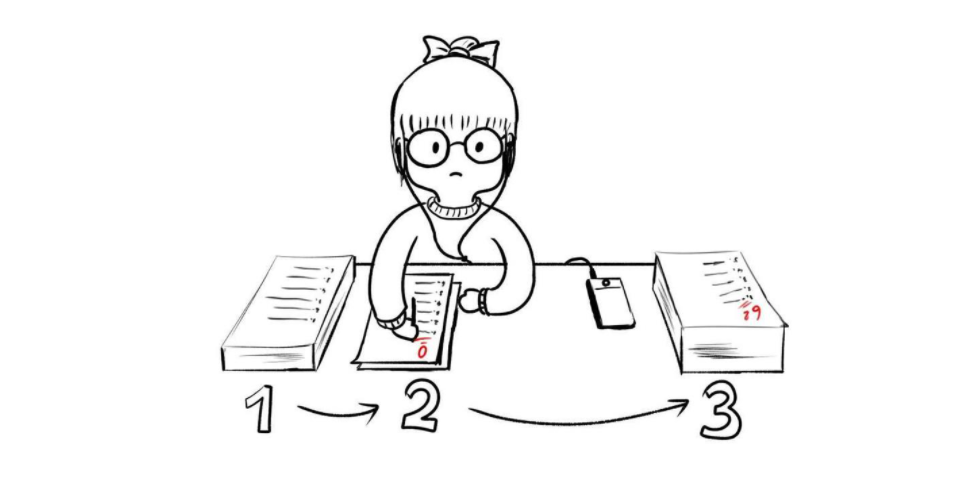
\includegraphics[width=7cm]{assets/Teacher_and_homework.png}
  \caption{老师和她需要批改的作业}
  \label{teacher-and-homework}
\end{figure}

老师批改作业的过程,可以简单地分解为下面这样几个步骤:

\begin{enumerate}
  \item 老师将这一摞作业堆在办公桌的一边,腾出办公桌的中央和另一边。
  \item 现在,老师取下这一摞作业中的一小叠,放在办公桌中央,开始伏案批改。
  \item 老师批改完了这一小叠作业,然后将它们放在办公桌的另一边,摞成新的一沓。
  \item 重复步骤 2 和步骤 3,最终老师完成了全部作业的批改,这时批改完的作业全部在在办公桌的另一边。
\end{enumerate}

我们会借助这个例子来更好地理解电脑硬件上的各个结构。

\subsection{处理器 / CPU}

中央处理器,简称「处理器」,英文简写「CPU」,是电脑内部最重要的一枚芯片,可以想象成是电脑的「大脑」。在上面的例子中,「老师」就相当于电脑中的处理器:「老师」的作用是对「作业」进行批改,从而完成教学任务;处理器的作用是进行各种的运算,从而实现电脑不同的功能。

你一定注意到过,电脑会发热——热到需要用一个风扇给它降温,这热量中有很大一部分就是处理器发出来的。如果你有关注过时事和新闻,中美贸易战中的「芯片」战,其中关键的一环就是处理器芯片。下图中,左为常见的台式电脑的 CPU 芯片,右为常见的笔记本电脑的 CPU 芯片。

\begin{figure}[H]
  \centering
  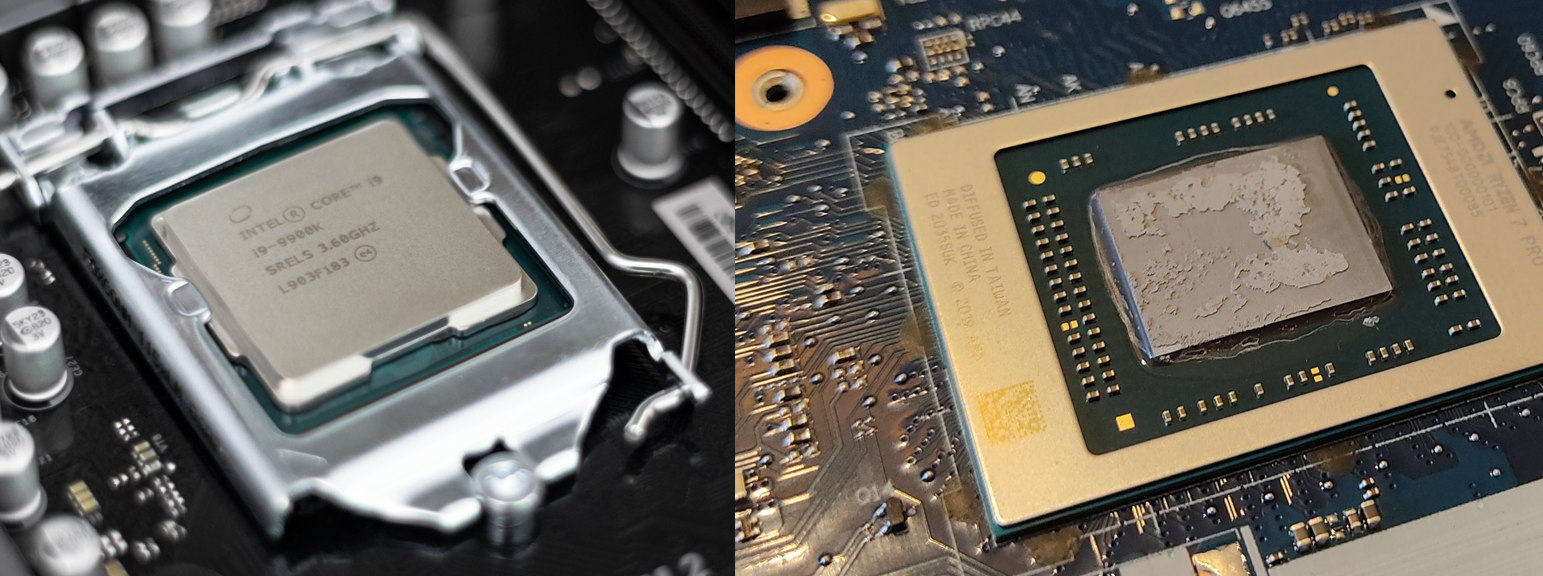
\includegraphics[width=10cm]{assets/CPUs.png}
  \caption{常见的台式机和笔记本电脑的处理器芯片。}
  \label{cpus}
\end{figure}

处理器是电脑工作的核心芯片,\regcolor{因此,处理器的性能就很大程度上决定了电脑的性能,决定了我们使用这台电脑流不流畅、玩游戏卡不卡、工作效率高不高}。在今天,全世界电脑芯片基本上是由两家美国公司设计制造\footnote{事实上,芯片的「设计」和「制造」两件事是不一样的,就像能设计出房屋的建筑师不一定会到工地上去砌墙。英特尔能够自行完成从设计到制造整条流水线,而 AMD 只能完成设计,它的处理器是由专门负责制造芯片的厂商(例如台积电)生产的。}的,其中一家叫做「英特尔」(Intel),另一家叫做「AMD」。

\begin{itemize}
  \item 英特尔公司现在主要的 CPU 产品线称作「酷睿」(Core),而「酷睿」系列又分成了 4 个档次——「i3」「i5」「i7」和「i9」。如果你现在在用笔记本电脑,不妨瞄一眼键盘下方是否有这样一个蓝色(也有可能是灰色,这里没有列出)的贴纸:
  \begin{figure}[H]
    \centering
    
\includegraphics[width=6cm]{assets/Stickers_Intel.png}
    \caption{英特尔的贴纸}
    \label{stickers-of-intel}
  \end{figure}
  \item AMD 公司现在主要的 CPU 产品线称作「锐龙」(Ryzen),而「锐龙」系列也分成了 3 个档次——「R5」「R7」和「R9」\footnote{其实还有 R3,但是很少在消费市场见到。}。如果你现在用笔记本电脑,不妨瞄一眼键盘下方是否有这样一个红色的贴纸:
  \begin{figure}[H]
    \centering
    
\includegraphics[width=2cm]{assets/Sticker_AMD.png}
    \caption{AMD 的贴纸}
    \label{sticker-of-amd}
  \end{figure}
\end{itemize}

我们常常说一个电脑是「双核」「四核」的,这里的「双核」「四核」也是处理器中的概念。这些处理器在一片芯片放了多个「核心」,相当于一个个协同起来的独立的小处理器。例如「双核」处理器,意味着在一枚处理器芯片上集成了两个核心,相当于两个大脑协同工作,当我们需要用电脑同时做很多事情的时候就有所裨益。同理,「四核」「八核」就是在一个芯片上集成了四个甚至是八个核心。

需要强调的是,\regcolor{并不是说核心数越多的处理器性能一定越好},更\regcolor{不是说 i7 处理器就一定比 i5 更好},也\regcolor{不是说英特尔的处理器就要比 AMD 好}。我们应该这样辩证地理解这些概念:每个品牌都有自己的不同系列,有的系列高端,有的系列低端;每个系列也都有自己的不同型号,有的型号性能强,有的型号性能弱。CPU 的性能并不与某一个因素呈线性的关系,而是多个因素综合的结果。

\subsection{内存 / RAM}

紧接着,我们介绍能直接与处理器交流的部件——内存,英文简写「RAM」。上一小节提到,处理器相当于大脑,但与大脑不同的是,处理器只能\regcolor{处理}数据,而这些待处理的数据,需要依赖外部的元件来临时存储。内存就是用来临时存储数据的。

内存本质也是一组芯片。生产内存这种芯片和生产处理器那种芯片所用的工艺有一些不同,目前生产内存这种芯片的厂商集中在韩国和中国台湾。一般这些芯片被排在条形的电路板上,这样的整体叫做「内存条」。下图中,上方的内存条是台式电脑使用的,下方的内存条是笔记本电脑使用的。

\begin{figure}[H]
  \centering
  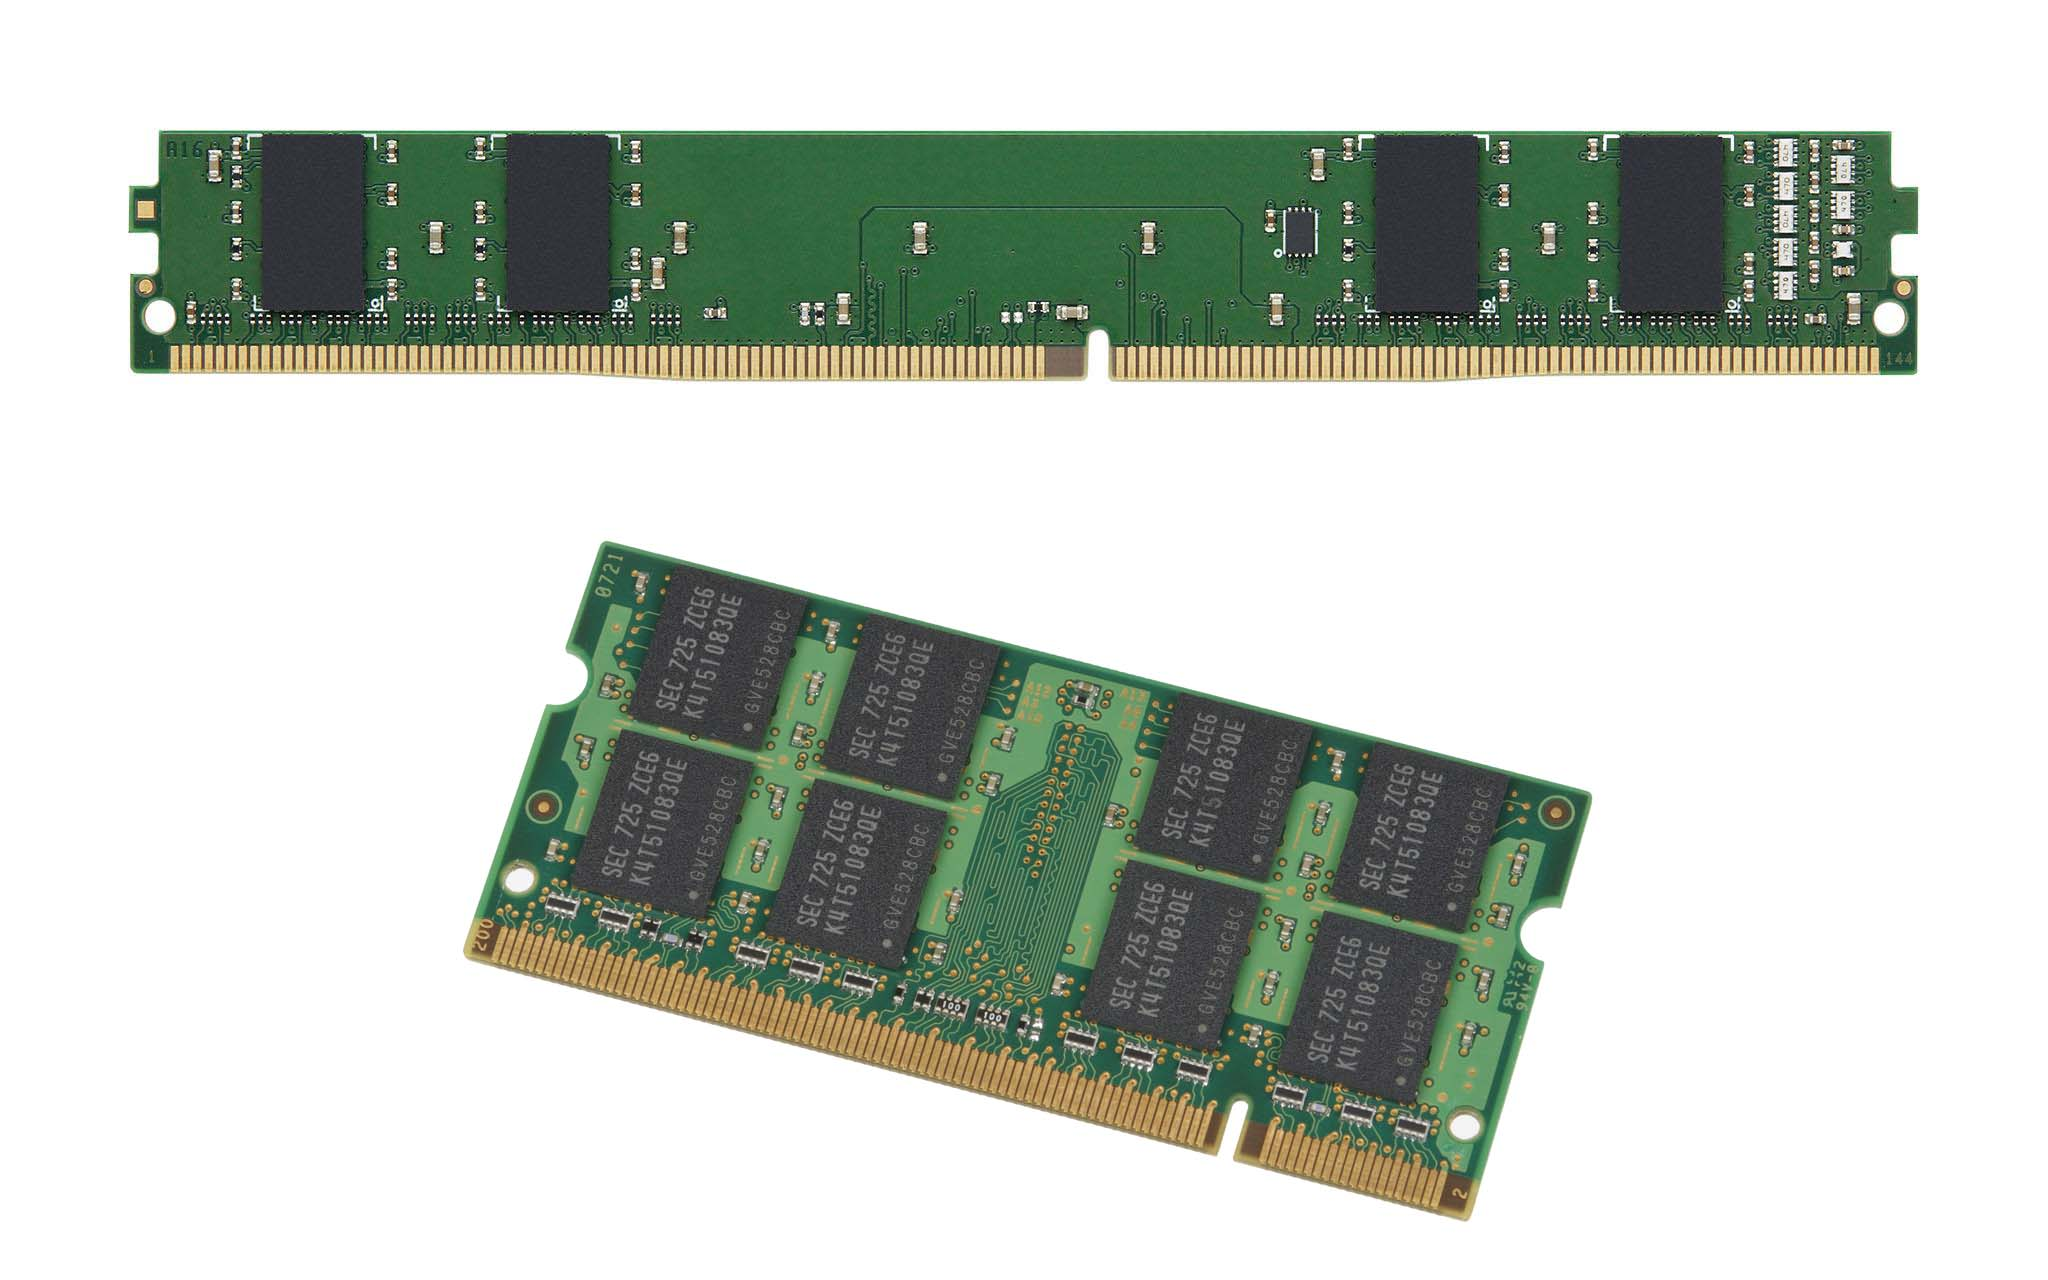
\includegraphics[width=8cm]{assets/RAMs.jpg}
  \caption{常见的内存条}
  \label{rams}
\end{figure}

前文说,内存直接与处理器进行数据交流。与处理器那极快的运算速度相匹配,内存的读取与写入速度也是极快的。但\regcolor{内存有一个特点——断电即丢失数据}。也就是说,当你电脑关机,内存中的数据便不复存在,又回到白纸一块。如果你想在内存里长久存放数据,那唯一的做法就是一直通电,多浪费电啊是吧。

回到前面老师批改作业的场景。办公桌的中央区域可以理解为「内存」:老师将作业放在办公桌中央批改,是因为这里改起来最方便;处理器将数据放在内存中处理,是因为这里读取和写入速度最快。办公桌中央不能总是放着东西,不然会弄乱、弄丢;内存中的数据一旦断电就会消失,因此总是临时的。

在 21 世纪初技术不是很发达的时候,内存的容量也不是很大,有 512 MB 已经不得了了。但随着时间的流逝,现如今大容量内存已经司空见惯。要想让现今的普通电脑基本流畅运行,内存容量应当至少有 4 GB。当然这东西倒是多多益善,就像更大的桌子能摆更多东西一样,\regcolor{更多的内存意味着更多的空间来让处理器存放数据,也就意味着电脑能同时处理更多的任务,基本意味着电脑更加流畅。}据我们的经验,流畅运行诸如 AutoCAD、Photoshop 之类的专业软件至少需要 8 GB 的内存。整体来说,在目前(2021 年),16 GB 的内存对于绝大多数人都已经够用了。

\begin{note}
  对应到手机中,内存有时会被手机厂商称为「运行内存」,不过我们不推荐如此称呼。
\end{note}

\subsection{硬盘}

内存是用来临时存储数据的,而硬盘则是用来长久保存数据的。与内存相比,硬盘的读写速度要慢得多,但存在硬盘中的数据不会因为断电而轻易消失,因此,\regcolor{硬盘是数据的最初的起点和最终的归宿}:处理器在一开始,从硬盘中取出数据放入内存,在内存中处理数据,处理完成之后,再将新的数据放回硬盘。

在前面老师批改作业的场景当中,办公桌两侧堆作业的地方可以理解为「硬盘」:大量的作业被堆在那里,整齐摆放,不会弄散、弄丢,但老师总是要把作业取到趁手的地方(办公桌中央)来批改;大量的数据被存在硬盘里,不会因为断电就丢失,但处理器总是要把数据放在快速的地方(内存)来处理。

简单来说,硬盘现在分为两种,一种叫「机械硬盘」(英文简称「HDD」)如下图左侧所示,一种叫「固态硬盘」(英文简称「SSD」)如下图右侧所。前者容量大、价格低、速度更慢,后者容量小、价格高、速度较快(但远远没有内存那么快)。前者是利用电磁原理存储数据,后者是芯片存储数据,但这种芯片和内存的那种又不一样——内存那种断电数据就消失了,固态硬盘的芯片断电还能保持数据。

\begin{figure}[H]
  \centering
  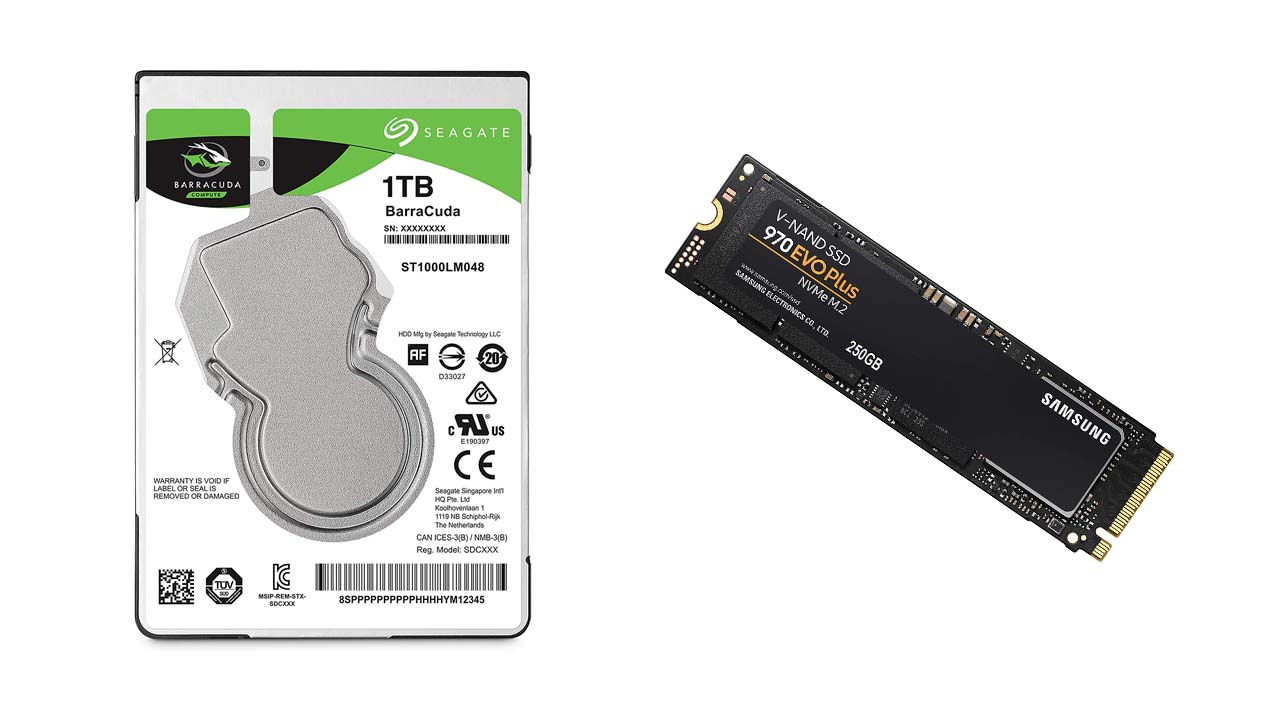
\includegraphics[width=8cm]{assets/Disks.jpg}
  \caption{常见的硬盘}
  \label{disks}
\end{figure}

在今天(2021 年),标称容量 512 GB 的固态硬盘大约 500 元,机械硬盘大约 200 元;标称容量 1 TB 的固态硬盘大约 800 元,机械硬盘大约 280 元。今天的中档次电脑常见的组合是用一块小容量(比如 256 GB)的固态硬盘,搭配一块大容量(比如 1 TB)的机械硬盘来实现各自功能的互补。稍微高档次一点的电脑,则会选用一整块更大容量(比如 512 GB 甚至 1 TB)的固态硬盘而不再使用机械硬盘。

打开桌面上的【此电脑】,你看到的所谓「C 盘」「D 盘」,就是硬盘上的空间——一块硬盘的空间可以被划分成不同的「盘」(学名叫「分区」)来更好地利用。

\begin{figure}[H]
  \centering
  
\includegraphics[width=10cm]{assets/Partition.png}
  \caption{打开【此电脑】,你就能看到硬盘的几个分区}
  \label{partitions}
\end{figure}


\regcolor{硬盘对电脑使用体验的影响,主要是「打开软件的速度」,包括「开机的速度」}。这是很容易理解的,因为数据原先都是存在硬盘里的,处理器从硬盘里「拿」数据的速度就直接影响着软件启动或者说加载的时间。

\begin{note}
  手机中也有类似固态硬盘一样的芯片来存储数据,它有时候被手机厂商称为「存储内存」,但它\regcolor{完全不是}内存。这是为什么有人会弄混「内存」和「硬盘」的根源之一。大家常说的「手机内存不够」,指的往往是存储空间(可以理解为「手机的硬盘」)不够,而不是真正的「内存」不够。
\end{note}

\subsection{显卡 / GPU*}

对于喜欢玩游戏的同学来说,「显卡」是他们在选购电脑时会着重考虑的一个因素。

最开始,「显卡」就是电脑里面的一个独立的芯片,像内存那样有自己的独立的电路板并插接在主板上。这个芯片的功能是专门进行画面的绘制和图像的处理,因而得名「显」卡。所有显示在屏幕上的画面,都是由显卡进行「绘制」的。因而\regcolor{显卡的性能主要是对游戏以及一些图形相关的工作(比如三维制图、视频剪辑)有较大影响}。下图是近 20 年前的电脑显卡的照片。

\begin{figure}[H]
  \centering
  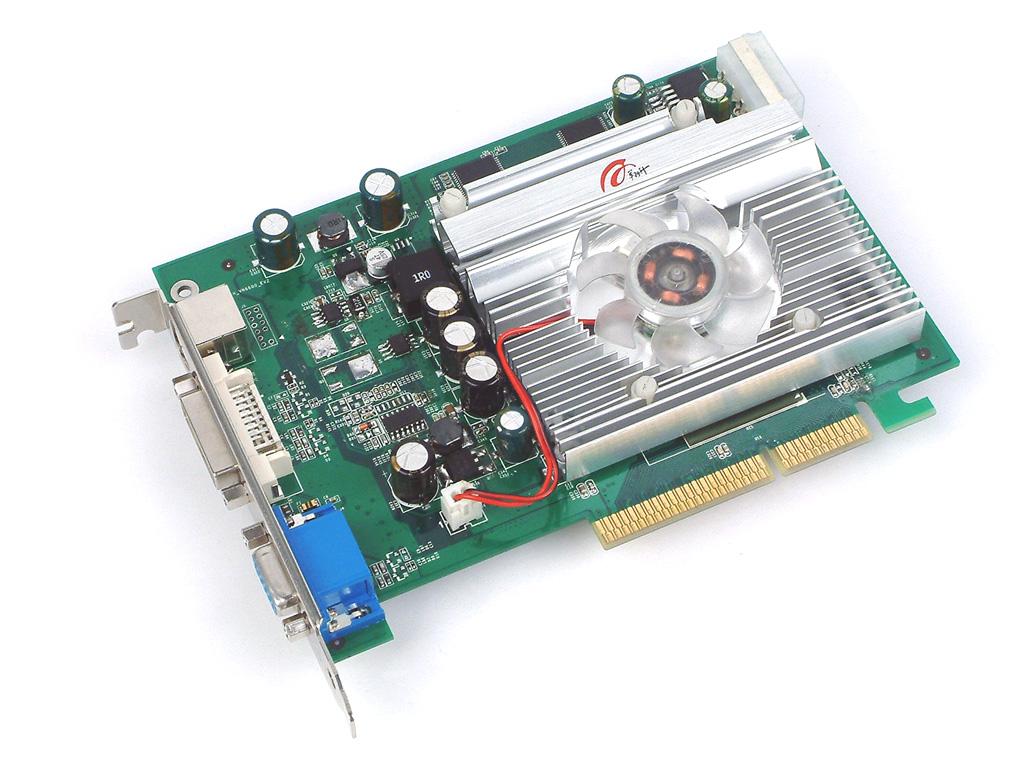
\includegraphics[width=8cm]{assets/Old_GPU.png}
  \caption{以前电脑上的显卡}
  \label{old-gpu}
\end{figure}

为什么上面那段要加上「最开始」三个字呢?因为随着半导体技术的发展,人们后来发现,显卡可以被「集成」到处理器\footnote{一开始,集成显卡并不是集成到处理器中的,而是集成在主板上的一个芯片之中(称为「北桥」),后来才集成到了处理器里面。}中,换言之,就像多核处理器把几个核心放在一个芯片上一样,显卡也可以和处理器放在一个芯片上。容易想到,这样集成到一起之后,显卡就不能做得很大了(受限于芯片整体的大小),也不能做得性能很强了(因为处理器核就在它边上,大家一起发热,一起分享能量),但可以缩小硬件的体积,也能降低功耗。因而,发展到今天,显卡在电脑中的形态有了以下两种:

\begin{itemize}
  \item \regcolor{集成显卡},英特尔称「核芯显卡」,AMD 称「APU」。显卡被安排在处理器的同一片芯片上,性能相对较差(但还是能应付大多数工作的,只是游戏、制图等特定工作就不太行了),功耗低,体积小。
  \item \regcolor{独立显卡},简称「独显」。显卡仍然是一片独立的芯片,有自己的供电和外围元件。这样的显卡性能比较强,但换来的是更高的功耗、更大的体积(游戏本为什么重)和更多的发热等。
\end{itemize}

\begin{figure}[H]
  \centering
  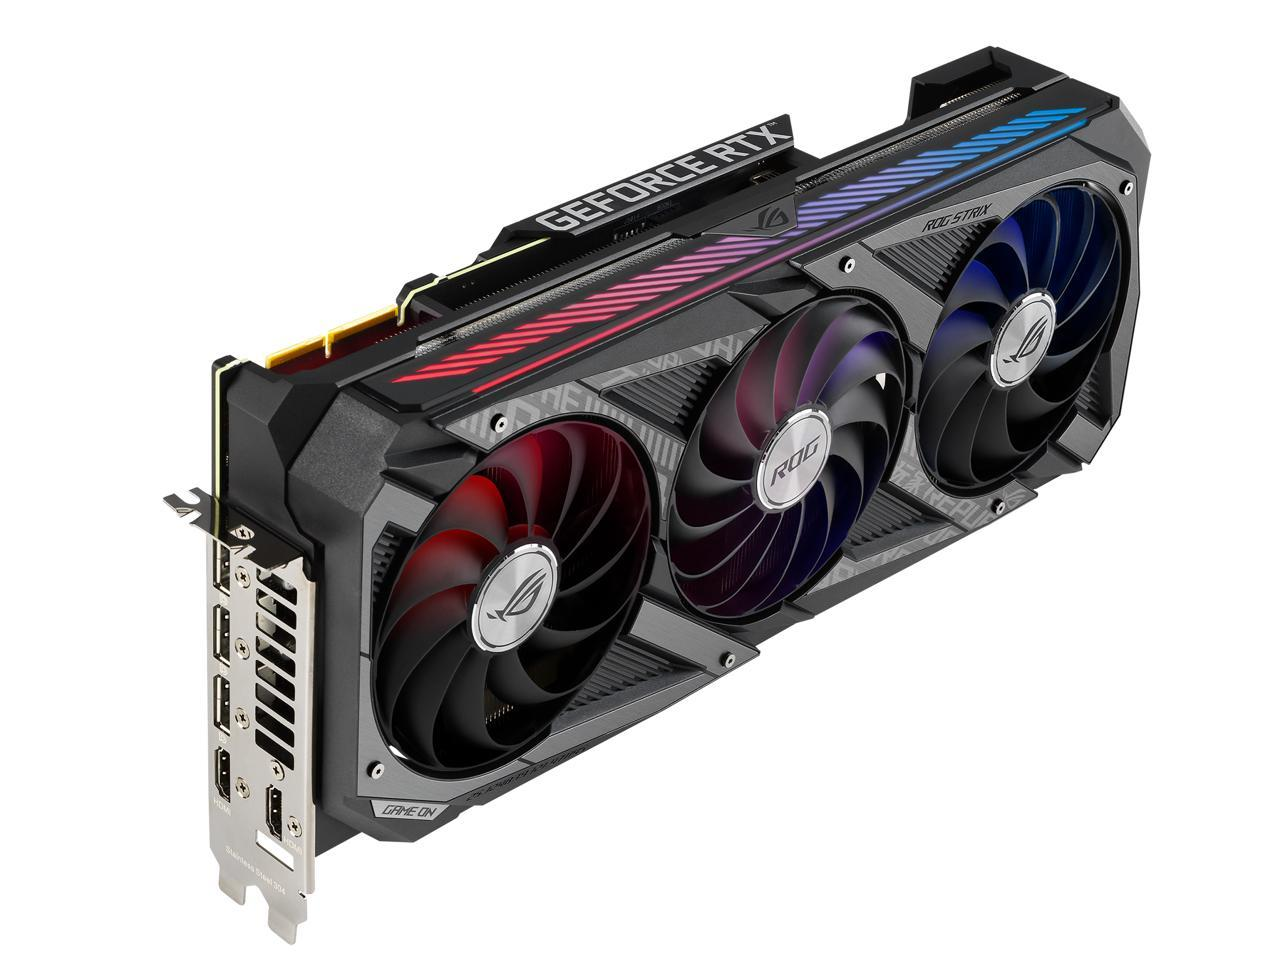
\includegraphics[width=8cm]{assets/3090.png}
  \caption{英伟达目前的顶级游戏显卡「RTX 3090」}
  \label{3090-gpu}
\end{figure}

今天,全世界生产\regcolor{独立显卡}的厂商主要有两家,一家叫「英伟达」(Nvidia),它生产的显卡俗称「N 卡」;另一家是前文提到过造处理器的「AMD」,它生产的显卡俗称「A 卡」。如果你有涉足过硬件交流圈,玩家所说的「RTX 3060」「GTX 1080 Ti」等都是英伟达显卡的型号,「RX 6800 XT」「RX 580」等都是 AMD 显卡的型号。上图是目前英伟达的顶级游戏显卡 RTX 3090。

\begin{note}
  是不是有人会问,那生产集成显卡的厂商有哪些呢?这个问题这里不回答,因为这不构成一个问题。
\end{note}


一般来说,对于笔记本,轻薄本都没有独立显卡而是使用集成显卡,游戏本都装配有独立显卡。这是由它们的使用场景和目标人群不同所决定的。

\section{与我们「打交道」的软件}

\subsection{软件与操作系统}

下面我们简单介绍「软件」和「操作系统」的概念。

由处理器、内存、硬盘以及各种各样的外围电子元件,共同构成了一台电脑的「硬件」部分。「硬件」就是电脑中电子电路的部分。而在「硬件」之上,硬件的具体工作任务是由「软件」来决定的。

我们用大家更熟悉的手机来做一个解释。\regcolor{手机上大家自己装的「QQ」「微信」「网易云音乐」,以及不是自己装的「电话」「短信」等 app 就属于「软件」}。「QQ」「微信」指导硬件去利用网络收发信息,利用屏幕展示数据,「网易云音乐」指导硬件去播放声音,同时在屏幕上展示评论,「电话」「短信」指导硬件利用无线电模块发送和接受信号……同样一部手机,硬件还是那个硬件,但能通过不同的软件行使不同的具体功能。

而在「QQ」「微信」「电话」等 app 之下,在纯粹的硬件之上,有\regcolor{一个更大、而且更「底层」的大软件,这个软件叫「操作系统」}。简单地说,操作系统「夹」在各个 app 和硬件之间,为 app 具体行使功能提供了一系列方便的「接口」。有了操作系统,网易云音乐的的开发者不再需要真正地去学习「怎么让喇叭发声」,而只需要学习「怎么告诉操作系统让喇叭发声」。「让喇叭发声」是一个带一些物理复杂知识的过程,但「告诉操作系统让喇叭发声」则相对简单得多。

\begin{figure}[H]
  \centering
  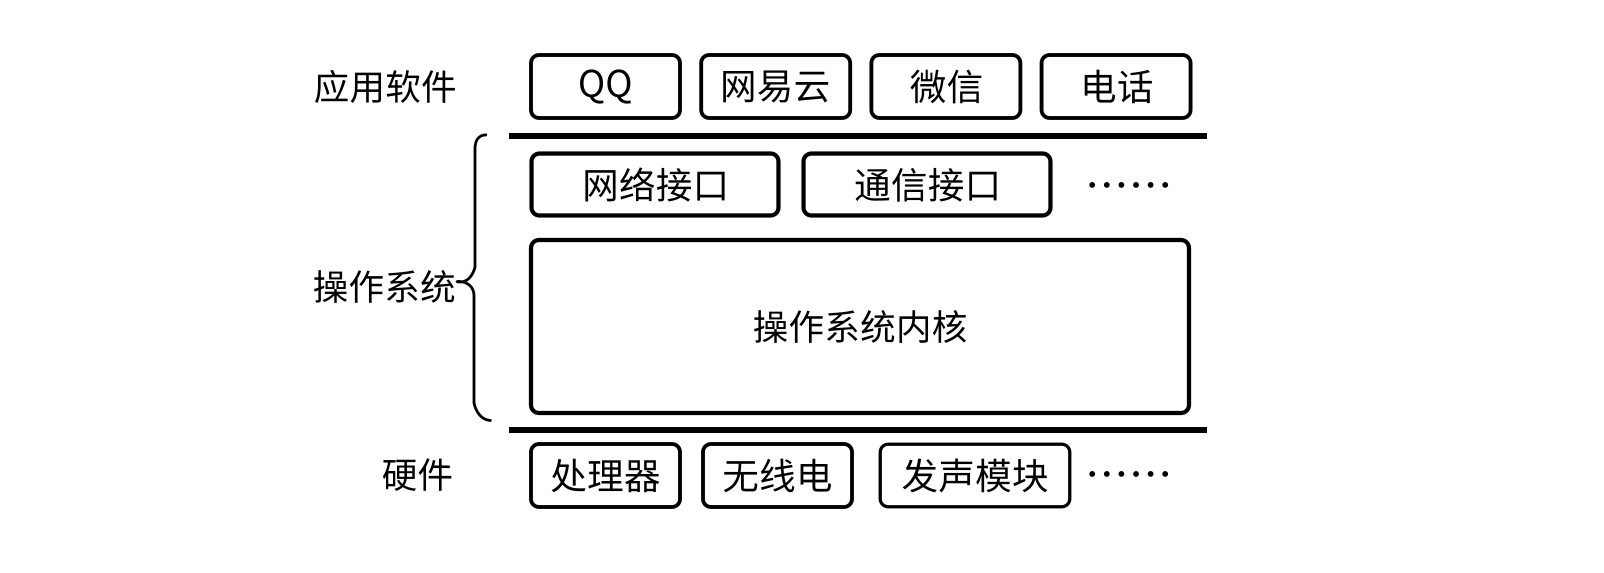
\includegraphics[width=10cm]{assets/Computer_Structure.png}
  \caption{App、操作系统和硬件的关系}
  \label{computer-structure}
\end{figure}

由于上层的软件(也就是 app)需要依赖操作系统来实现功能,而每个操作系统留给 app 的接口细节上有不同,因此,针对不同操作系统开发的软件是不能直接通用的。App 厂商一般会为不同的操作系统开发同一款 app,这样就能照顾到使用不同系统的用户。

今天主流的手机操作系统有「安卓」(Android)和「iOS」。后者只能使用在 Apple 的硬件上,前者则被各个手机厂商使用\footnote{华为开发的「鸿蒙」(Harmony OS)由于以某种方式兼容安卓软件,在这里我们暂且作为前者对待。}。而到了电脑上,「Windows」和「macOS」是最常见的两种操作系统。后者只能使用在 Apple 的硬件上。由于我们认为 macOS 的使用者不会依靠《Missing》来学习电脑知识,因而《Missing》中的所有操作都是认定读者使用 Windows 系统的。

下图中,左侧是 Windows 操作系统的典型界面,而右侧是 macOS 系统的典型界面。

\begin{figure}[H]
  \centering
  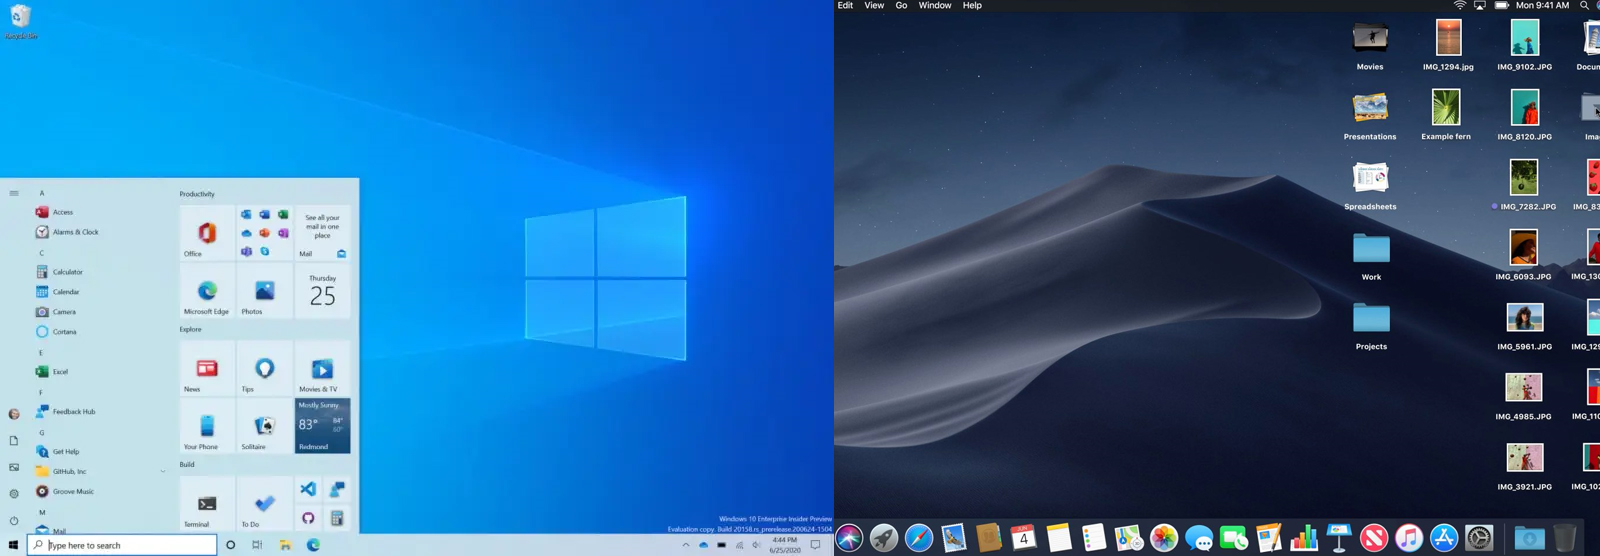
\includegraphics[width=10cm]{assets/Windows_and_macOS.png}
  \caption{Windows 和 macOS 系统的界面}
  \label{win-and-mac}
\end{figure}

\subsection{Windows 操作系统}

我们的大多数人使用的都是 Windows 操作系统。所谓「Windows XP」「Windows 7」和「Windows 10」则是 Windows 操作系统的不同版本。

Windows 由美国的微软公司(Microsoft)所开发,诞生于 1985 年。到今天(2021 年),Windows 已经经历了数个大版本的更新。目前最新的 Windows 版本是「Windows 11」(发布于 2021 年 10 月 5 日),我们大多数人使用的是「Windows 10」,还有一些稍旧的计算机在使用「Windows 7」。更老的 Windows 版本,例如「Windows XP」,已经鲜有使用。不同版本 Windows 系统之间会有操作细节、使用体验上的不同,不过往往最直观的不同是它们的「外观」。

Windows 可以使用在英特尔或者 AMD 处理器的电脑上——事实上,今天除了 Apple 以外几乎所有品牌的个人电脑都运行着 Windows 系统。通过右键桌面上的【此电脑】并点选【属性】,你可以看到自己电脑 Windows 系统的版本。

\begin{figure}[H]
  \centering
  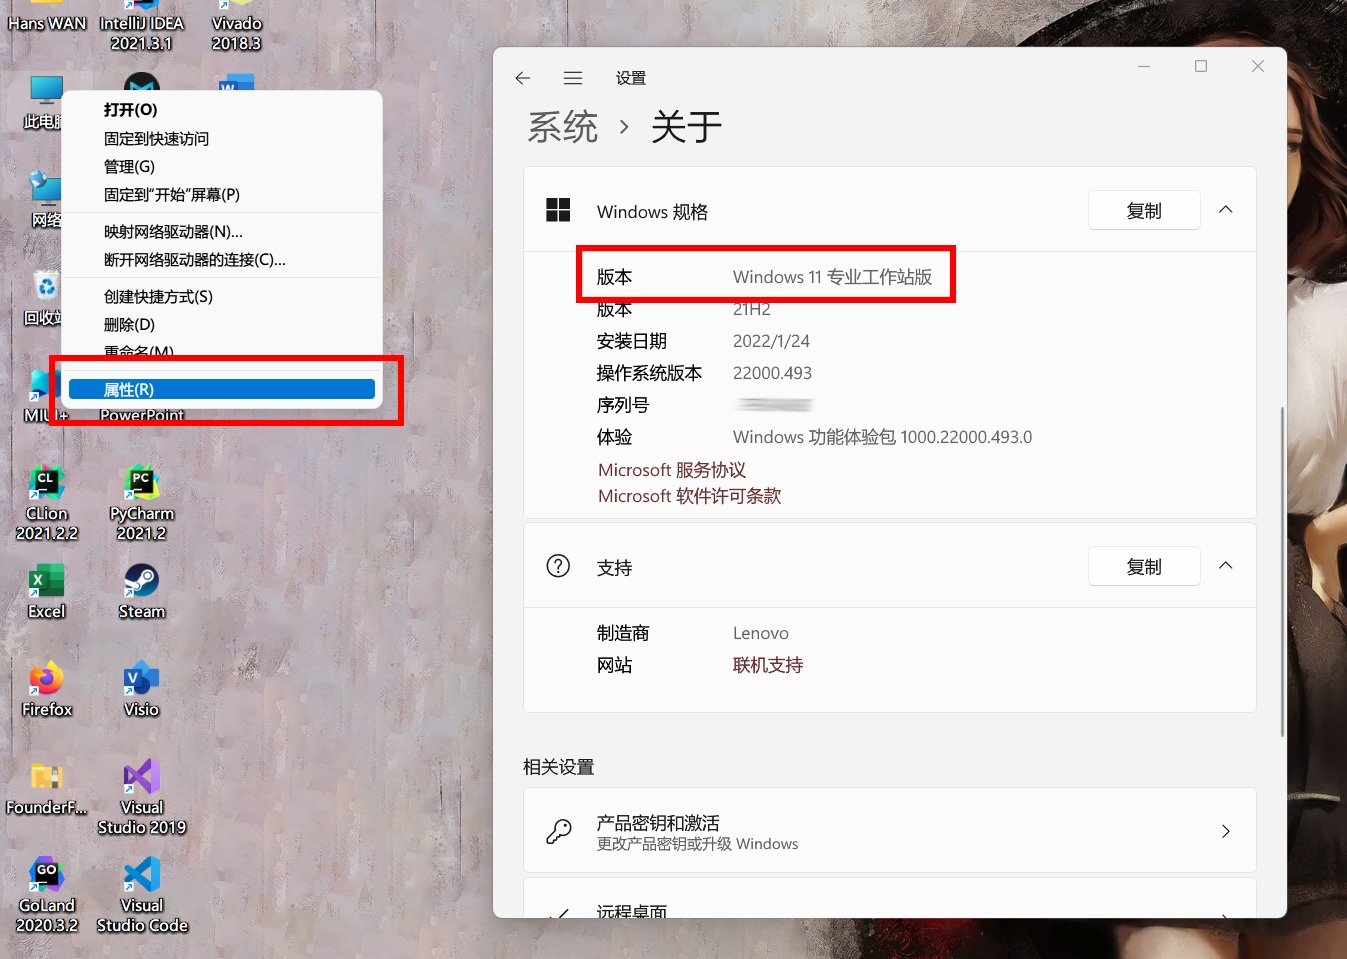
\includegraphics[width=8cm]{assets/Check_Windows_version.png}
  \caption{检查 Windows 系统的版本}
  \label{check-windows-version}
\end{figure}

《Missing》假定读者使用的系统是 Windows 10 或者 Windows 11,其中所有的操作都是基于 Windows 10 或者 Windows 11 简体中文版系统来描述的。如果你使用的是 Windows 7、Windows 8 或者 Windows 8.1,其中大多数操作也都能正常使用。一些明确仅能用于 Windows 10 和 / 或 Windows 11 的操作和技巧会被标注。

\practice

\begin{enumerate}
  \item 在之前打开的【此电脑】→【属性】,你除了能看到自己电脑的 Windows 版本之外,也能找到自己电脑的处理器型号和内存容量信息。尝试去查找这个信息,并自行上网搜索你的处理器型号,辨认它的品牌、系列,判断它是几核处理器,「主频」有多高。(「主频」是描述 CPU 性能的一个指标。)
  \item 你使用的是游戏本还是轻薄本?亦或是介于二者之间的所谓「全能本」?尝试翻到笔记本的底面,上网搜索它底面所写的型号,了解关于你自己机器的更多信息。
  \item 在 Windows 10 / 11 中,打开【任务管理器】,切换到【性能】选项卡,可以看到一个更详细的硬件运行状态,其中【硬盘】相关栏目展示了你设备的硬盘数量和类型(机械硬盘 HDD、固态硬盘 SSD)。尝试查看你电脑的硬盘容量和类型。
  
  你可以通过按 \keys{Ctrl} + \keys{Shift} + \keys{Esc} 来打开「任务管理器」。也可以右击【开始按钮】,选择【任务管理器】来打开它。
  \begin{figure}[H]
    \centering
    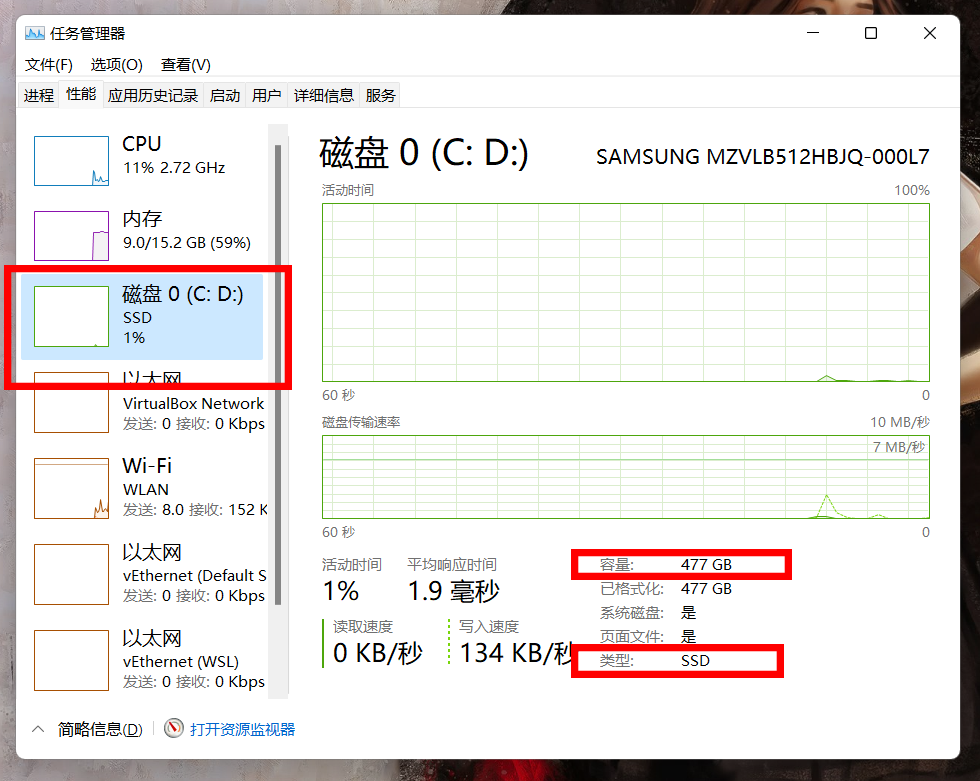
\includegraphics[width=8cm]{assets/Check_disk_status.png}
    \caption{查看电脑硬盘容量和类型}
    \label{check-disk}
  \end{figure}
  \item 你对「电路」的认知有多少?你是否好奇 CPU 是怎么运作的?从开关、导线、电池、灯泡组成的最简单「电路」到几乎无所不能「电脑」之间到底发生了什么奇妙的变化?《Missing》限于篇幅是不可能告诉你这些的。但是,你若有兴趣,可以去学习「电路电子技术」「数字电路与数字逻辑」「计算机体系结构」等相关内容。近年来,国际形势风云变幻,我国在芯片领域仍然存在许多短板。我们希望越来越多的有志青年能投身于包括但不限于体系结构、硬件组成、数字电路乃至微电子、半导体材料等领域,为我国芯片行业「补上短板」贡献自己的力量。
\end{enumerate}

\chapter{文件与文件管理}
\label{files-and-file-management}

\begin{intro}
  在这一部分,我们将重新介绍你可能所不知道的「文件」以及「文件」的管理,以及一些实用的文件管理的技巧。
  看完这一部分,你将可以找到下面这些问题的答案:
  \begin{itemize}
    \item 为什么很多人说「不建议把文件放在桌面上」?
    \item C 盘总是「红了」,为什么?为什么有人建议把软件装到 D 盘里?
    \item 「扩展名」是什么?「打开方式」又是什么?为什么有时候我电脑上的 Word 文档就打不开了?
  \end{itemize}
\end{intro}

如上一章所言,硬盘是电脑中存放数据的地方,而「文件」则是数据存放的具体形式。
你所撰写的 Word 文档、制作的 PPT 幻灯片、从网上下载的图片,乃至各个 app 或者说软件本身,都以文件的形式存储在硬盘上。

这一部分,我们将具体介绍「文件」和文件的管理。
这是《Missing》需要动手实践的第一章,也是我们合理、有效地使用电脑的第一课。

\section{硬盘的分区}

打开桌面上的【此电脑】,我们往往可以看到多于一个的「盘」,例如 C 盘、D 盘等。
这样的「盘」学名叫做「分区」,顾名思义,它们是将硬盘上的空间人为地划分成了一些子空间。

\begin{figure}[htb!]
  \centering
  
\includegraphics[width=13cm]{assets/Hans_Disks.png}
  \caption{Hans 电脑上的分区}
  \label{Hans_Disks}
\end{figure}

例如,上图是 Hans 的笔记本电脑「此电脑」中的分区。
可以看到,这两个分区一个大小为 175 GB,另一个大小为 299 GB,相加为 474 GB——这是这台电脑的硬盘可用总空间。

划分分区的意义,在于帮助我们更好地管理文件。
分区划分之后,各个分区之间就仿佛被「隔离」开来了,如图 \ref{Disk_Parts} 所展示的那样。
即使我们「格式化」一个分区(这样会删除这个分区中的所有文件),也不会影响另外一个分区里面的文件。

\begin{figure}[htb!]
  \centering
  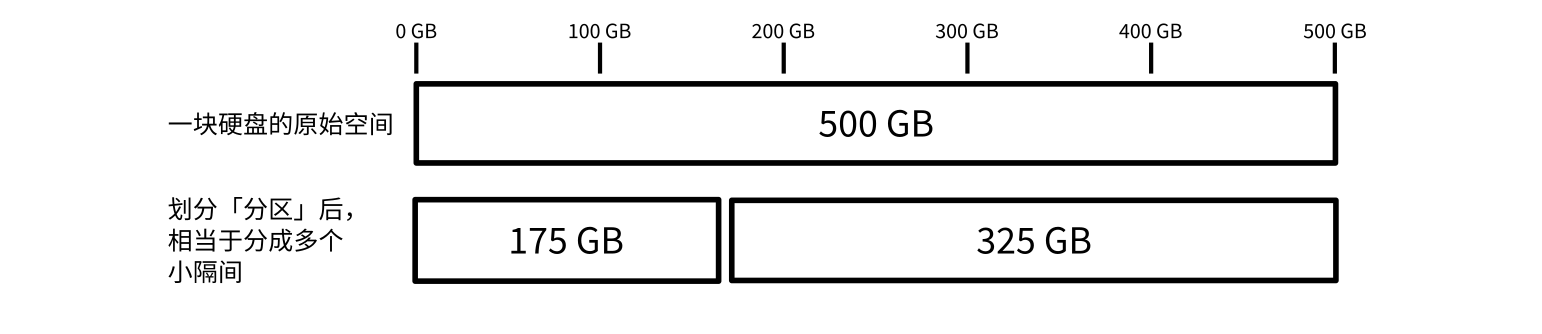
\includegraphics[width=12cm]{assets/Disk_Parts.png}
  \caption{硬盘与分区的关系}
  \label{Disk_Parts}
\end{figure}

在 Windows 系统中,分区会被给予两个标识符,或者说「名字」:

\begin{itemize}
  \item 一个是「\regcolor{盘符}」,盘符是一个英文字母加上冒号 \verb|:| 构成的。
    我们所称呼的「C 盘」「D 盘」正是指盘符中的那个字母。
    如上图,左方分区的盘符是 \verb|C:| ,右方分区的盘符是 \verb|D:| 。
    盘符一般在被指定之后就不方便更换了。在今天,Windows 系统中的盘符都是从字母 C 开始\footnote{这是因为 A 和 B 两个盘符在过去是留给「软盘」的,但软盘早就已经成为历史了,不过这个习惯却保留了下来。}的。
  \item 另一个是「\regcolor{卷标}」,这是一个可选的标识符,它是一定长度的文本。
    在上图中,C 盘的卷标是「Windows」,D 盘的卷标是「Files」。
    盘符的作用是让系统和软件识别分区,而卷标的作用是帮助我们用户更加直观的了解分区的作用,因而卷标是可以随时更换的。
    事实上,通过右键某一分区,选择【重命名】,就可以更换卷标了。如果你什么都不写,它默认叫做「本地磁盘」。
\end{itemize}

\begin{figure}[htb!]
  \centering
  
\includegraphics[width=7cm]{assets/Volume_Name_and_Letter.png}
  \caption{盘符与卷标}
  \label{Volume_Name_and_Letter}
\end{figure}

我们在\nameref{computer-and-its-components}中提到,操作系统本身也是一个大软件,那么这个软件放在硬盘上的哪呢?
对于 Windows 而言,整个 Windows 系统默认放在 C 盘里。
双击打开电脑 C 盘,你会看到一些你可能不熟悉的文件夹,例如 \verb|Windows| 文件夹,Windows 系统自己的许多文件就存在其中。

也许你听过「不要把软件安装到 C 盘」这样的说法。这是有根据的。
系统本身就已经很庞大,系统自身工作产生的一些文件也会被自动地放在 C 盘内,导致 C 盘本身空间就容易变得局促。
如果还将大量的软件装在 C 盘,会让 C 盘更加「不堪重负」,结果就是——红了。

在本章的后续部分,以及\nameref{software-installation}中,我们会详细介绍,怎样把我们的软件以及其他东西放在 C 盘以外的地方,以及这样做的其他好处。

\section{文件、文件名和和文件类型}

「文件」是数据存储在硬盘上的形式。这么说可能有些抽象,直观地说,文件就是我们每天都打交道的东西:

\begin{figure}[htb!]
  \centering
  
\includegraphics[width=7cm]{assets/Files.png}
  \caption{一些文件}
  \label{Files}
\end{figure}

文件有自己的「名字」,称为「文件名」。
在 Windows 系统中,文件名可以分成三个部分:

\begin{itemize}
  \item 「主名」是指文件名中,点号 \verb|.| 之前的部分。
    这部分内容可以自定,相当于人类的姓名。
    上图中,「 \verb|如何让富婆爱上我| 」和「 \verb|一夜暴富指南| 」等都是文件的主名。
  \item 「点号」是指文件名中间的那个「 \verb|.| 」。
  \item 「扩展名」是指文件名中,点号「 \verb|.| 」之后的部分\footnote{有时候我们称呼文件的扩展名时也会把点号包含进去。下面两种说法是等价的:
      \begin{itemize}
        \item 某文件的扩展名是\texttt{txt}。
        \item 某文件的扩展名是\texttt{.txt}。
      \end{itemize}}。
    扩展名展示着文件的类型,它会告诉操作系统,这个文件应该用什么方式来打开。
    例如,上图中「 \verb|每天一个长寿秘诀.txt| 」中的「 \verb|txt| 」就是这个文件的扩展名,它说明这个文件是一个「文本文档」,应该使用「记事本」打开。
\end{itemize}

\begin{figure}[htb!]
  \centering
  
\includegraphics[width=5cm]{assets/File_Name.png}
  \caption{文件名结构}
  \label{File_Name}
\end{figure}

扩展名也是可以人为改变的,但这样往往会出问题——试想,对于上图中的 \texttt{高等数学不挂速成.mp4} ,它本来是一个 \verb|mp4| 文件,即「视频文件」,应该用看视频的软件打开。
如果你强行把它改成 \verb|txt| ,系统就会用「记事本」来打开一个「视频文件」——用错误的工具打开文件。

如果你的电脑上,文件的扩展名没有被显示(也就是说你只能看到文件的主名),像这样:

\begin{figure}[htb!]
  \centering
  
\includegraphics[width=5cm]{assets/Files_No_Ext.png}
  \caption{没有显示扩展名的文件}
  \label{File_No_Ext}
\end{figure}

在 Windows 10 中请点选文件夹窗口上方的【查看】选项卡,然后勾选【文件扩展名】,如图 \ref{Windows_10_set_full_filename} 所示;在 Windows 11 中请点选文件夹窗口上方的【查看】菜单,然后勾选【显示】→【文件扩展名】,如图 \ref{Windows_11_set_full_filename} 所示。

\begin{figure}[htb!]
  \centering
  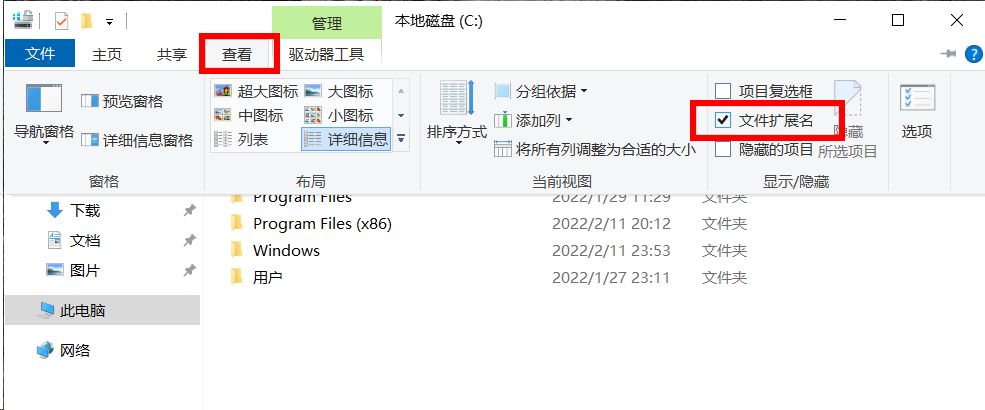
\includegraphics[width=10cm]{assets/Windows_10_set_full_filename.png}
  \caption{Windows 10 设置方法}
  \label{Windows_10_set_full_filename}
\end{figure}

\begin{figure}[htb!]
  \centering
  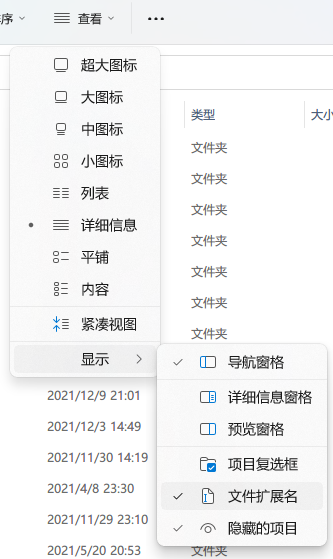
\includegraphics[width=4cm]{assets/Windows_11_set_full_filename.png}
  \caption{Windows 11 设置方法}
  \label{Windows_11_set_full_filename}
\end{figure}

在打开这个选项之后,文件扩展名不仅是可见的,甚至是可以改变的——但如上文所说,扩展名不能随便改,因为改了之后系统就会用错误的工具去打开它。
右键某一文件,选择【重命名】,你会看到系统会自动帮你选中文件的「主名」,而不选中「扩展名」。
如果你执意更改文件的「扩展名」,系统会发出一个提示:

\begin{figure}[htb!]
  \centering
  
\includegraphics[width=6cm]{assets/Warning_of_Changing_Ext.png}
  \caption{尝试更改扩展名……}
  \label{Warning_of_Changing_Ext}
\end{figure}

\section{文件夹、路径和目录}

「文件夹」是一个用来存放其他文件的结构。
不妨想象一下现实中的「文件夹」:

\begin{figure}[htb!]
  \centering
  
\includegraphics[width=4cm]{assets/Real_Folder.png}
  \caption{真实的文件夹}
  \label{Real_Folder}
\end{figure}

在这样的一个「文件夹」中,可以放很多各类「文件」。
而电脑中的文件夹除了能放文件之外,还可以放很多的「子文件夹」,即「文件夹里面的文件夹」。
这个过程可以循环重复,因而一个文件夹的内部结构可以相当错综复杂。

如果抽象地把整个电脑看成一个巨大的「文件夹」,那么不同的分区就是这个巨大「文件夹」之下的几个子文件夹,我们的某一份文件就是在这些子文件夹之下的某一个角落里。
假设在 D 盘的 \verb|missing| 文件夹之中有一个叫做 \verb|源文件| 的子文件夹,在这个子文件夹中有一个文件叫 \verb|第三章.docx| ,我们用这种方式表示这个 \verb|第三章.docx| 文件在整个电脑中的位置:

\begin{verbatim}
  D:\missing\源文件\第三章.docx
\end{verbatim}

这一长串东西表示出 \verb|第三章.docx| 这个文件在电脑中的具体位置,我们把一长串东西称为 \verb|第三章.docx| 这个文件的「路径」(严格来说叫做「绝对路径」)。
不难发现,路径是从「分区」(也就是「盘」)开始,用反斜杠 \verb|\| 作为分隔,一级一级文件夹地展开,最后到具体的文件。
类似的,不只是文件,文件夹的路径也可以用这样的方式来表示,例如

\begin{verbatim}
  D:\missing\源文件
\end{verbatim}

表示的就是 \verb|源文件| 这个文件夹在电脑中的位置。
一个文件 / 文件夹的「路径」是唯一确定的;一个「路径」也能唯一确定一个文件 / 文件夹。

也许你有听说过「目录」这个名字。其实「目录」就是文件夹。
例如这个说法「打开目录 \verb|D:\missing\public\| 」 指的就是打开 D 盘中 \verb|missing| 文件夹里的 \verb|public| 文件夹。

目录(文件夹)一层一层的结构可以像图 \ref{Catalog_Tree} 一样从上到下画出来,称作「目录树」。
在目录树这种形式中,文件夹之间是「上下级」的关系,故「文件 A 在文件夹 B 中」也可以称作「文件 A 在文件夹 B 下」或者「A 在目录 B 下」甚至是「A 在 B 下」。
也就是说,「下」这个字就是「在……里」的意思。

\begin{figure}[htb!]
  \centering
  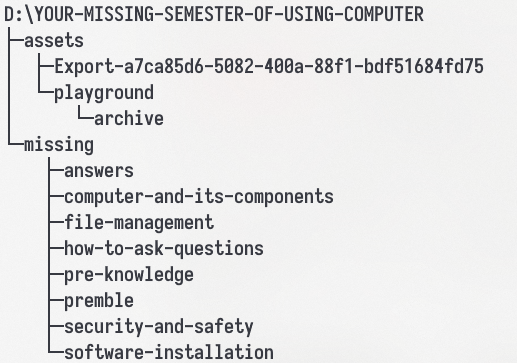
\includegraphics[width=8cm]{assets/Catalog_Tree.png}
  \caption{目录树}
  \label{Catalog_Tree}
\end{figure}

借助目录树这样的结构,我们就能理解「根目录」这个概念了。
一个盘的「根目录」指的是这个盘之下的第一级目录(恰好是目录「树」的「根」),例如 C 盘根目录就指的是路径 \verb|C:\| 。

\section{程序本身——可执行文件(\texttt{exe}文件)}

这一节我们介绍一种类型特殊的文件——「可执行文件」。
我们提到,数据是以文件的形式存储在硬盘上的,比如你所撰写的 Word 文档,它们都存储成了扩展名为 \verb|doc| 或者 \verb|docx| 的文件;
你所下载的图片,它们的扩展名则往往是 \verb|jpg| 、 \verb|png| 或者 \verb|gif| 。
而我们又提到,软件或者说 app 也是以文件的形式存储在硬盘上的。
那么,软件本身是什么格式的文件呢?

一个软件的核心是一个或多个「程序」,而程序是以「可执行文件」的形式存储的。
\regcolor{普通的文件,需要用其他的某个软件才能正常打开;而「可执行文件」双击就能运行自身,这就是「可执行」(Executable)的意思。}

可执行文件的扩展名是 \verb|exe| 。
对于这种类型的文件,系统不会想着用别的软件去打开它,而是直接运行它自身。
可执行文件有时被直接成为「程序文件」或者「程序」。

需要注意的是,电脑上的一款软件(或者说 app,在《Missing》中我们会同时使用这两种称呼)可能不仅仅只有一个程序,也就不止有一个可执行文件。
下面是软件「网易云音乐」所在的文件夹中的一部分:

\begin{figure}[htb!]
  \centering
  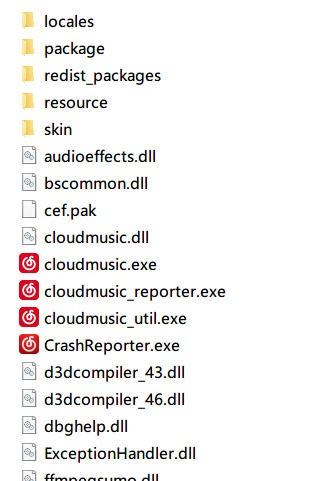
\includegraphics[width=5cm]{assets/NetEase_Music.png}
  \caption{网易云音乐的目录}
  \label{NetEase_Music}
\end{figure}

可以看到,「网易云音乐」这个 app 有着这些文件:

\begin{itemize}
  \item 可执行文件 \verb|cloudmusic.exe| ,这个是 app 的主体,即「网易云音乐」的主程序。
  \item 可执行文件 \verb|cloudmusic_reporter.exe| , \verb|cloudmusic_util.exe| 等。
    这些文件是 app 运行时的其他辅助程序,可以想象成乐队中主唱身边的吉他手 / 键盘手 / 鼓手 / 伴舞等。
    它们往往无法单独运行,而 \verb|cloudmusic.exe| 这个主文件脱离它们也不能运行。
  \item 一大堆的 \verb|dll| 和其他格式的文件。这些是 app 工作时不可或缺的依赖文件。
  \item 一些子文件夹,存储着 app 运行需要的另外一些东西。
\end{itemize}

每次我们启动「网易云音乐」,运行的都是 \verb|cloudmusic.exe| 这个可执行文件。
然而,这个文件的运行离不开放在它边上的那一堆辅助文件——如果你把 \verb|cloudmusic.exe| 复制到另外的一个地方,双击运行,大概率会直接报错;即使不报错,功能也必然有不正常。

在下一章我们在介绍软件的安装时会继续说明这个问题。

\section{文件的「替身」——快捷方式}

你是怎么启动「网易云音乐」的呢?

一般来说,我们会双击桌面上的「网易云音乐」或者点击开始菜单中的「网易云音乐」。
不管是桌面上的「网易云音乐」还是开始菜单里的「网易云音乐」,它们都是不是这个 app 本身——app 本身的样子我们在上面刚刚看过——而是另一种特殊类型的文件,称作「快捷方式」。

\begin{figure}[htb!]
  \centering
  
\includegraphics[width=10cm]{assets/Shortcut.png}
  \caption{快捷方式}
  \label{Shortcut}
\end{figure}

「快捷方式」可以看成某个具体文件的单向「指针」或者说「替身」,指向电脑某个角落里的某个文件。
它的扩展名是 \verb|lnk| ,但实际上不可见\footnote{千万不要手动把一个正常文件的扩展名改成\texttt{lnk},否则就很难改回来了。}。
你桌面上的「网易云音乐」,指向的正是网易云音乐软件目录下的那个 \verb|cloudmusic.exe| 文件。右击桌面上的【网易云音乐】,选择【属性】,会弹出这个快捷方式的详细信息:

\begin{wrapfigure}[12]{r}{6cm}
  \centering
  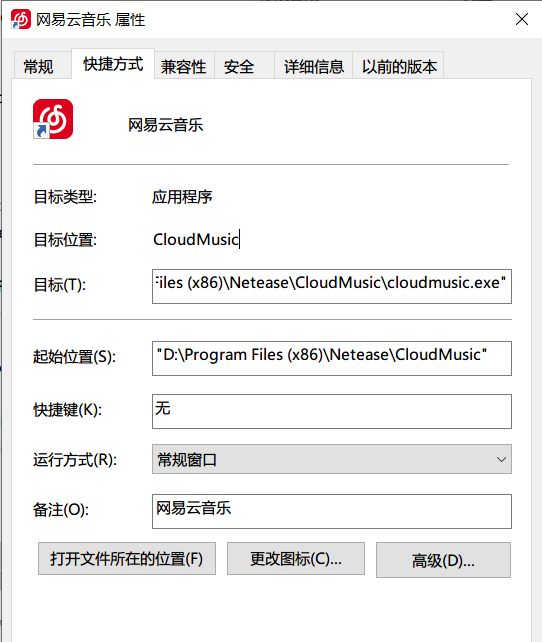
\includegraphics[width=5cm]{assets/NetEase_Music_Link.png}
  \caption{桌面上的「网易云音乐」}
  \label{NetEase_Music_Link}
\end{wrapfigure}

其中「目标」一栏填写的正是 \verb|cloudmusic.exe| 这个可执行文件,即「网易云音乐」的主程序的路径:

\begin{verbatim}
  D:\Program Files (x86)\Netease\CloudMusic
  \cloudmusic.exe
\end{verbatim}

因此,你双击打开这个「网易云音乐」快捷方式,就会打开 \verb|cloudmusic.exe| 这个文件。
如果你\regcolor{删掉了这个快捷方式,它并不会影响 \texttt{cloudmusic.exe} 这个文件,不会影响你电脑上安装的网易云音乐本身。}

\begin{note}
  因此,卸载软件的方式可不是把桌面上的「快捷方式」删掉就完事的。
\end{note}

所有类型的文件以及文件夹都可以制作出无数个快捷方式。
如果你想给自己的某个文件 / 文件夹制作一个快捷方式,只需右键它,选择【发送到】→【桌面快捷方式】,就能在桌面生成一个指向这个文件的快捷方式了。
这个快捷方式可以挪到系统的任何地方,也可以复制粘贴出很多个副本。它们全都指向原来的那个文件本身。

一般来说,快捷方式的图标左下角会有一个「↗」符号。
这个符号标志着这个文件并非某文件本身而是一个快捷方式。

\section{合多为一,精简空间——压缩文件}

压缩文件并不是什么「特殊类型」的文件,但这里我们依然把它单独拿出来介绍。

压缩文件是利用一种特殊的软件「压缩软件」,将一批文件和文件夹「打包」而成的一种单个文件。
假设你有 8 个文件夹以及 7 个文件一共 15 个项目,你想一次性把它们分享给别人,那么把它们打包成一个压缩文件不失是一种好的选择。

\begin{figure}[htb!]
  \centering
  
\includegraphics[width=10cm]{assets/Compress.png}
  \caption{普通文件与压缩文件}
  \label{Compress}
\end{figure}

压缩文件有很多种类。最常用的是 \verb|zip| 文件和 \verb|rar| 文件,但后者的压缩软件是收费的\footnote{具体来说,大多数压缩工具都可以解压 \texttt{rar} 格式的压缩包,但只有 WinRAR 这一款压缩工具可以制作这种格式的压缩包;而这款工具是收费的。详见\nameref{archive-formats-and-tools}。}。
我们建议在与他人交换文件的时候,只使用 \verb|zip| 格式打包。

如果你电脑上已经安装有压缩软件,那么可以参照下面的方法将一批文件打包成一个压缩包:


\begin{itemize}
  \item 选中你要打包的文件。可以使一个文件 / 文件夹,也可以是一群文件 / 文件夹。
  \item 右击,选择【添加到压缩包】或者类似语义的选项。
  \item 设置参数,例如压缩格式(推荐 \verb|zip| 格式)、压缩后的文件的文件名以及压缩方式。\\
    一般来说,压缩后的文件的体积要比原来松散文件的体积小(所谓「压缩」)。
    具体而言,在压缩时可以选择「更快压缩」和「更小体积」之类的选项,前者压缩、解压都更快,但压缩时体积缩小的不明显;后者压缩、解压相对较慢,但压缩后体积可能缩小得更多。
  \item 开始压缩。压缩完成后,在原来的文件的相同目录下,就会生产一个 \verb|<文件名>.zip| 的文件。
\end{itemize}

如果收到一个压缩文件,我们一般需要将它解压。如果你电脑上已经安装有压缩软件,那么可以参照以下方法来解压缩:
右击压缩文件,选择【解压\footnote{部分压缩工具称「解压」为「提取」,是同一个词(Extract)的不同翻译。}到当前文件夹】或者【解压到 \verb|<文件名>\| 】。这两个选项的不同是:

\begin{itemize}
  \item 【解压到当前文件夹】会把压缩文件里的内容直接放在压缩文件的同一目录下。
    例如,如果一个压缩文件 \verb|archive.zip| 里面有 \verb|a.txt| 和 \verb|b.txt| 两个文件,选择此选项,解压后 \verb|a.txt| 和 \verb|b.txt| 都和 \verb|archive.zip| 在同一级目录。 
    \begin{figure}[htb!]
      \centering
      \begin{minipage}{6.2cm}
        \centering
        
\includegraphics[width=6cm]{assets/Decompress_Current.png}
        \caption{【解压到当前文件夹】}
        \label{Decompress_Current}
      \end{minipage}
      \qquad
      \begin{minipage}{6.2cm}
        \centering
        
\includegraphics[width=6cm]{assets/Decompress_Sub.png}
        \caption{【解压到\texttt{<文件名>\textbackslash}】}
        \label{Decompress_Sub}
      \end{minipage}
    \end{figure}
  \item 【解压到 \verb|<文件名>\| 】会把压缩文件里的内容放在一个子文件夹里面。
    在上面的例子中选择这个选项,会在 \verb|archive.zip| 的同一级目录新建一个文件夹 \verb|archive| ,然后把 \verb|a.txt| 和 \verb|b.txt| 放在 \verb|archive| 文件夹下。
\end{itemize}

我们建议,为了不让自己的工作目录变得混乱,\regcolor{除非你知道自己这样做的原因,否则使用「提取到\texttt{<文件名>\textbackslash}」}。

如果我们只是想查看一个压缩文件的内容,而不把它解压,或者只提取出压缩文件中的一个文件,在系统装有压缩软件的情况下可以直接双击打开压缩文件。
直接双击打开压缩文件,压缩软件会展示出其中的内容。
双击这里面的单个文件可以临时取出这一个文件并打开它,拖拽其中的单个文件到其他地方可以只取出这一个文件而不解压整个压缩文件。

有关压缩格式和压缩软件以及它们的使用的更多细节,请参见\nameref{archive-formats-and-tools}。

\section{文件的打开方式}

在前文中说到,不同类型的文件需要用不同的 app 来打开。
对于一个特定的文件类型,打开它的 app 称为它的「打开方式」。
如果「打开方式」不对,就会出现问题。

容易想到,Word 文档 \verb|doc| 和 \verb|docx| 文件的打开方式就是 Word 软件或者 WPS 软件;图片 \verb|jpg| 、 \verb|png| 等的打开方式就是各种看图软件;PDF 文档 \verb|pdf| 的打开方式就是 PDF 阅读器软件,例如 Acrobat 或者 SumatraPDF……

\begin{note}
  可执行文件的打开方式是什么呢?
  这个问题这里不作回答,因为这不构成一个问题。
\end{note}

系统内部维护有一张「表」,这个「表」记录了已知的文件类型(扩展名)和对应的打开方式。
你可以把这张表想象成这样:

\begin{table}[htbp]
  \centering\begin{tabular}{*{3}{>{\small}c}}
    \toprule
    扩展名 & 用什么软件打开 & 软件主程序的路径在哪 \\\midrule
     \verb|txt|   & 记事本 &  \verb|C:\Windows\system32\notepad.exe|  \\
     \verb|docx|  & Word &  \verb|C:\Program Files\Microsoft Office\root\Office16\WINWORD.EXE|  \\
     \verb|mp3|  & 网易云音乐 &  \verb|D:\Program Files (x86)\Netease\CloudMusic\cloudmusic.exe|  \\
    …… & …… & …… \\\bottomrule
  \end{tabular}
  \caption{简易的「表」}
  \label{regtable}
\end{table}

有了这张表,系统就能自动地帮我们选择文件对应的打开方式。
有时,我们不想要用这张表帮我们预置的方式来打开文件。
比如,打开 \verb|jpg| 图片的默认方式是「图片」软件,但如果我们想\regcolor{暂时}用「Photoshop」来打开它,我们可以这样做:

\begin{itemize}
  \item 右键要打开的这个 \verb|jpg| 文件,选择【打开方式】,在里面选择【Adobe Photoshop】。
    \begin{figure}[htb!]
      \centering
      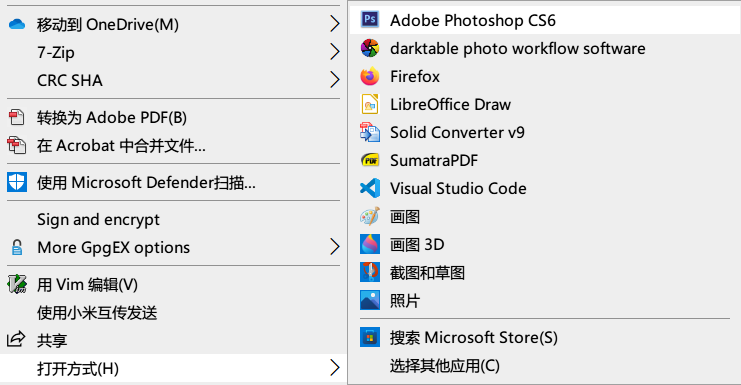
\includegraphics[width=9cm]{assets/Select_Open_with.png}
      \caption{更改打开方式}
      \label{Select_Open_with}
    \end{figure}
  \item 如果上一步找不到「Adobe Photoshop」,那么选择【打开方式】→【选择其他应用】。
    然后在弹出的对话框中寻找【Adobe Photoshop】,点击并选择【确定】。
    注意\regcolor{不要}勾选「始终使用此应用打开 \verb|.jpg| 文件」。
    \begin{figure}[htb!]
      \centering
      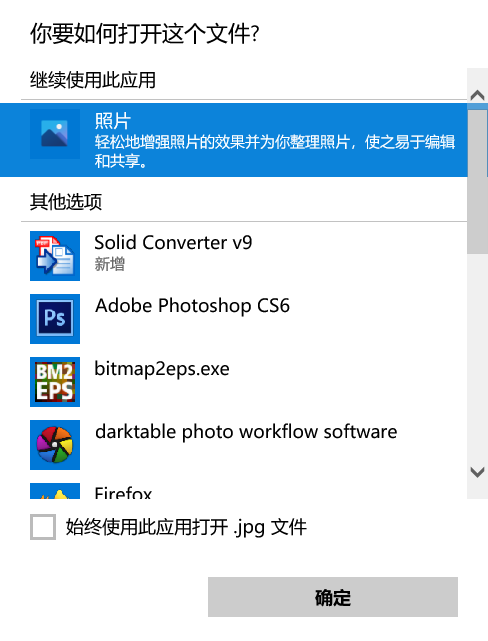
\includegraphics[width=5cm]{assets/Open_with.png}
      \caption{进一步选择}
      \label{Open_with}
    \end{figure}
  \item 如果上一步还找不到「Adobe Photoshop」,而你确实电脑上装有 Photoshop,那么可能需要手动找到 Photoshop 的那个可执行文件,也就是它的 \verb|exe| 文件。
    这个文件的路径——也就是软件的安装路径——在下一章我们会提到。
    一般来说是在 \verb|C:\Program Files| 或者 \verb|C:\Program Files (x86)| 之下的某个文件夹中。
\end{itemize}

\regcolor{如果你想永久地指派某一文件的打开方式,则可以在上面步骤的基础上,勾选【始终使用此应用打开 \texttt{xxx} 文件】。}
这样,系统内部的那张「表」就会被更改,系统以后都会用你指派的新应用来打开这种文件。

除了你手动更改之外,这张「表」还可能在这些情况被更改:

\begin{itemize}
  \item 系统安装更新,即 Windows Update 之后,这张表可能会被重置而丢失一些项目,造成某些文件突然无法打开。这往往是由于你使用的对应软件并不是原版,而是某种「精简版」所造成的。
  \item 新安装一个软件时,软件安装程序可能写入新的表项,来为即将安装的新软件的文件类型配置打开方式。
  \item Windows 的各种恶性 bug 和恶心操作。例如,Windows 会时不时用 Microsoft Edge 代替其他软件来打开网页文件和 \verb|pdf| 文件等。\CJKsout*{(微软你坏事做尽)}
\end{itemize}

如果你的文件关联某天突然失效,即某种类型的文件突然无法打开,但对应的软件工作正常,那么可以考虑是否是上面的原因。

\section{管理好你的文件}

管理好我们的文件,不外乎两个方面:

\begin{itemize}
  \item 对自己的文件进行整理归类。比起将所有文件「随手乱放」,如果我们将自己的文件按它们的性质、类别等归类存放,必然有助于提升我们的工作效率。
  \item 不把(重要)文件放在 C 盘。在前文我们说了,C 盘是 Windows 系统整个所在的地方。
    尽管发生这种情况的概率很低,但当我们的电脑因为这样或那样的原因损坏,而需要重装系统的时候,你会不得不失去 C 盘的所有文件——安装系统的第一步就是格式化 C 盘。
    让自己的文件远离 C 盘,是合理管理我们的文件的重要部分。
\end{itemize}

\subsection{为文件安家}

首先为你要放的文件选择一个合适的位置。

桌面,以及 Windows 系统预置的那些文件夹(「文档」「视频」「图片」等,打开【此电脑】就可以直接看到),除非按照后文所介绍的方法更改位置,否则全部是 C 盘内部的空间,因此在你手动更改它们的位置之前,\regcolor{不建议}将自己的文件放在这些地方。

另一方面,非 C 盘的分区,例如 D 盘甚至后续更多的磁盘分区,都是可以考虑的存放自己资料的位置。

找到一个合适的位置后,我们便可以建立一套自己的分类方法来对文件进行整理和分类。


\begin{itemize}
  \item 例如你有一些「学习资源」,你便可以在 D 盘或是什么别的盘建立一个名为「学习资源」的文件夹,再在其下——无论是按学科(例如「高数」「线代」「物理」),还是按时间(例如「大一上」「大一下」)——建立更多的子文件夹,来为它们进行更为详尽的分类。
  \item 再例如你有许多「大片」,你也可以按照地区、上映时间甚至是主演什么的为它们分类。
    不过鉴于大片不仅是名气大,占用空间也大,我们推荐腾出一个分区(甚至是一块硬盘)来存放它们。
\end{itemize}

总的来说,\regcolor{「为你的文件进行合理分类」}与\regcolor{「将你的硬盘进行合理分配」}便是这里的核心思想。

\subsection{定期打扫}

电脑里面的东西总是随着我们的日常使用而越积越多 \CJKsout*{(这里点名 QQ 的 \texttt{FileRecv} 和 \texttt{Image} 文件夹,藏得又深,又乱七八糟;还有微软的更新,一更一大堆)},所以定期检查你不需要的东西然后扔掉它们显得尤为重要。

对于系统分区 C 盘来说,你不去动它,它也会被塞入一些诸如系统临时文件、Windows 更新文件等等这些。
我们推荐新手用户们运用一些诸如「火绒安全软件」「360 电脑管家」之类的 app 中的清理功能进行文件的清理。

但是上述软件并不会把我们日常中积累的用户文件(例如你收到的课件、文档等)也清理掉,但在日常使用过程中,我们也会不可避免地产生许许多多的冗余文件,或是曾经需要而现在不再需要的文件。
这里不妨就来看看上文所讲的那个 \verb|FileRecv| 文件夹:

\begin{itemize}
  \item 这个文件夹默认位于 \verb|文档\Tencent Files\<QQ 号>\| 处,每个不同的 QQ 号都有一个属于自己的个人文件夹。
    如果你没有按照后文「更改用户文件夹的存储位置」迁移「文档」文件夹的话,这东西也在 C 盘里,因为「文档」是在 C 盘里的;
  \item 点开 \verb|FileRecv| ,你在使用 QQ 的过程中接收到的所有文件都在此处,其中通过手机发给电脑的文件存储于专属子文件夹 \verb|MobileFile| 中;
  \item 将 \verb|FileRecv| 文件夹中的所有文件检查一遍,有用的就如上文所述归类、无用的则直接删除,这就大功告成了。
\end{itemize}

事实上 QQ 为用户提供了更改用户个人文件夹位置的功能,但是似乎更改的时候并不会将你曾经接收的文件一并移走,着实不好用,这里并不推荐。

同样地,在你已经归好类的文件体系中,也要时不时进行检查,删去冗余与无用文件,这样能够保持你的文件系统简而精。
《礼记·大学》载:「苟日新,日日新,又日新。」如是而已。

\subsection{更改用户文件夹的存储位置*}

上文提到了一个叫做 \verb|文档| 的文件夹,它是系统预置的一个用户文件夹。
在介绍这一部分之前,我们先简单提一下「用户文件夹」是什么。

如前所言,Windows 系统默认为用户准备了几个文件夹来进行文件的分类。
通过双击桌面上的【此电脑】,展开【文件夹】折叠项,你可以看到这些文件夹:

\begin{figure}[htb!]
  \centering
  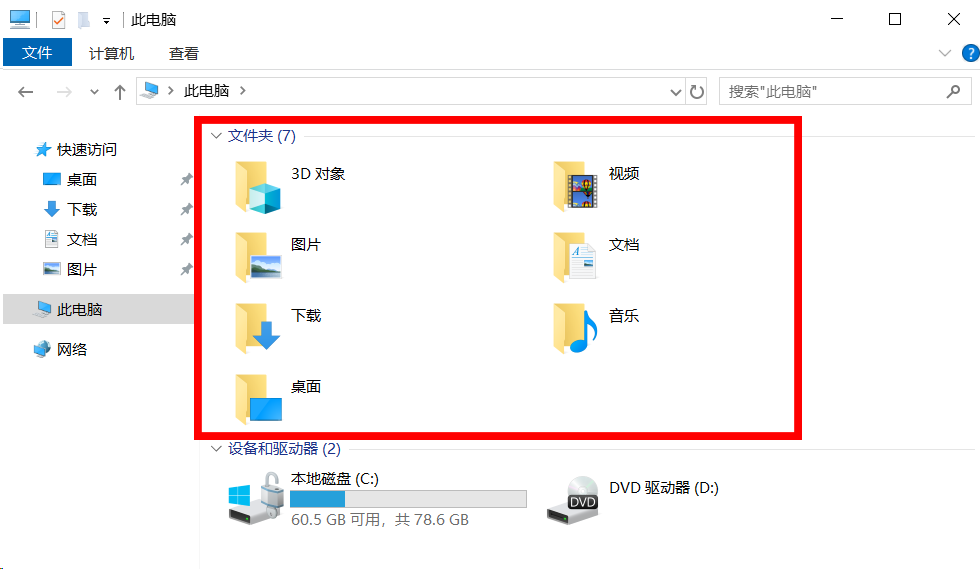
\includegraphics[width=11cm]{assets/User_directories.png}
  \caption{用户文件夹}
  \label{User_directories}
\end{figure}

Windows 系统的本意,是希望用户可以借助这些文件夹来辅助进行文件的整理。
可是,这些文件夹默认情况下全部位于 C 盘(路径是 \verb|C:\用户\<你的用户名>\| ),而把大量的个人文件放在 C 盘是我们所不建议的。
那这些系统「好心」准备给我们的文件夹就都不能使用了吗?
答案是否定的——通过迁移这些文件夹到 D 盘,我们可以在利用好这些用户文件夹的同时,保证自己的数据安全和系统稳定。

\begin{note}
  看到这几个文件夹中的「桌面」,你是否会有点奇怪?桌面为什么也是这里的一部分呢?
  事实上,桌面的本质也是一个用户文件夹。桌面上你放的文件、各个 app 的快捷方式都在这个文件夹中。
\end{note}

我们打开 \verb|C:\用户\<你的用户名>\| 可以看到全部的用户文件夹。
这些文件夹涵盖了「桌面」「文档」「图片」「音乐」「视频」等多种类别,并且都配有形象的图标,如图:

\begin{figure}[htb!]
  \centering
  
\includegraphics[width=5cm]{assets/All_User_Directories.png}
  \caption{更多用户文件夹}
  \label{All_User_Directories}
\end{figure}

我们的目的是把这些文件夹「迁移」到 D 盘(或者其他的某个磁盘,这里以 D 盘为例)。
这样,我们就可以充分地利用系统预置的这一批用户文件夹了。

右击某个我们想要迁移的文件夹(比如【桌面】),选择【属性】,然后切换到【位置】选项卡,如图:

\begin{figure}[htb!]
  \centering
  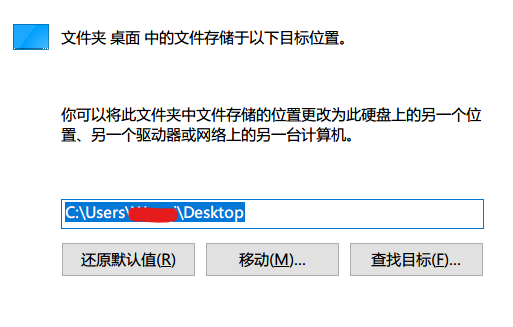
\includegraphics[width=8cm]{assets/Change_Directories.png}
  \caption{更改用户文件夹位置}
  \label{Change_Directories}
\end{figure}

我们将这里文本框中

\begin{verbatim}
  C:\Users\<你的用户名>\
\end{verbatim}

这一部分\regcolor{(注意:最后一个\texttt{Desktop}、\texttt{Documents}之类的名字不要动!)}\footnote{如果你不小心把一个用户文件夹的位置设置成了某个磁盘的根目录(比如说\texttt{D:\textbackslash}),会触发 Windows 系统的一个 bug,导致很难再改回来。\CJKsout*{(辣鸡 Windows)}}改成

\begin{verbatim}
  D:\
\end{verbatim}

\regcolor{也就是说,对于「桌面」而言,改完之后的完整路径是}

\begin{verbatim}
  D:\Desktop
\end{verbatim}

例如:

\begin{figure}[htb!]
  \centering
  
\includegraphics[width=8cm]{assets/Destination.png}
  \caption{填入目标位置}
  \label{Destination}
\end{figure}

点击【应用】,提示「文件夹 ‘D:\textbackslash{}Desktop’ 不存在,是否新建该文件夹」,选择【是】。

紧接着提示「是否要将所有文件从原位置移动到新位置」,选择【是】。

一般来说移动操作很快就会完成。完成后,点击【确定】。
这样「桌面」文件夹就被成功地迁移到了 D 盘。
你可以打开 \verb|D:\桌面| 来查看其中的内容,与你桌面上真正看到的东西应该大同小异。

\begin{note}
  对于桌面而言,现在你放在桌面上的文件本质上就存在 D 盘里了。
  但我们依然不建议你在桌面上放太多文件——因为这样不方便你自己寻找。
\end{note}

\regcolor{强烈建议进行迁移的用户文件夹有:}\regcolor{「文档」「桌面」「下载」。}

\regcolor{建议进行迁移的用户文件夹有:}\regcolor{「视频」「图片」「音乐」。}

迁移完成之后,你可以在迁移之后的位置(比如 D 盘)看到这些文件夹。
它们现在不在原来的 \verb|C:\用户\<你的用户名>\| 那里了。

\begin{figure}[htb!]
  \centering
  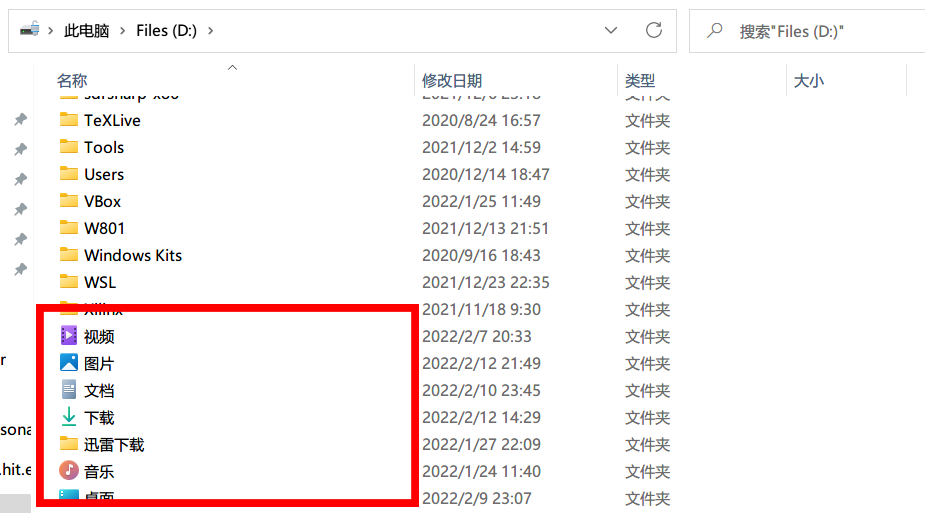
\includegraphics[width=12cm]{assets/Moved_user_directories.png}
  \caption{新的用户文件夹位置}
  \label{Moved_user_directories}
\end{figure}

\practice

\begin{enumerate}
  \item 查看自己电脑的几个分区的「卷标」,并依照自己的文件分类习惯修改成自己所喜欢的名字。例如,叫「资料」或者「Files」就比「新加卷」或者没有卷标(会显示「本地磁盘」)要直观得多。
  \item 尝试把一个图片文件的扩展名改成 \verb|txt| ,然后用「记事本」打开它。你看到了什么?\textit{记得改回来哦!}
  \item 试着迁移用户文件夹到 D 盘或者其他非 C 盘的分区,然后利用这些用户文件夹帮助自己整理文件。\\
    注意迁移的时候千万看清楚目标路径是完整的 \verb|D:\Documents| 、 \verb|D:\Desktop| 这样的路径,而不是光秃秃的一个 \verb|D:\| 。
  \item 整理你的 QQ 文件接收文件夹 \verb|FileRecv| 。
  \item 选择你自己的几个文件和文件夹,把它们打包成一个压缩文件 \verb|MyArchive.zip| ,复制到其他的某个地方,尝试两种不同的解压方式「提取到当前位置」「提取到 MyArchive\textbackslash{}」。
  \item 创建一个文档(可以是纯文本文件 \verb|txt| 或者 Word 文档 \verb|docx| 等)并写入一些内容,然后制作它的两个快捷方式,并把这两个快捷方式放在两个与源文件都不一样的地方。试着双击打开那两个快捷方式,你发现了什么?删掉两个快捷方式中的一个,源文件被删除了吗?
    另一个快捷方式还在吗?
\end{enumerate}
\chapter{软件的寻找与安装}
\label{software-installation}

\begin{intro}
  软件的下载安装一直以来是困扰许多「电脑小白」的大问题——从哪里下?怎么下?下完怎么装?装完怎么办?什么,软件要收费?破解是什么?……这一章将对国内互联网环境下 Windows 软件的下载、安装和配置做一个简单的介绍。看完这一部分,你或许可以找到下面这些问题的答案,并慢慢对「怎么寻找软件」有一个初步的了解。
  \begin{itemize}
    \item 我想下载 xxx 软件,我应该去哪里找这软件?
    \item 网上全是病毒和垃圾软件,我应该怎么样最大程度保证自己电脑的安全?
    \item 为什么软件下到手还要安装?有的还要破解?为什么这么麻烦?
    \item 电脑里不是有个「Microsoft Store」吗?为什么那里面大多数软件都找不到?
  \end{itemize}
\end{intro}

直到今天,Windows 系统下依然没有一个广泛使用的集中化「应用商店」。与我们使用手机不同,在电脑上,我们若想安装某个软件,多数情况下需要到互联网上寻找软件的「安装包」,再自行将软件「安装」到电脑上来使用。

这部分,我们将具体介绍软件为什么要「安装」,如何从网上的万千垃圾软件中下载我们需要的软件,以及软件安装和配置的一些技巧和注意事项。

\section{安装与安装包}

在 Windows 系统上,应用是通过「安装包」来安装到系统上的。如果把 app 比作是一株植物,那安装包就是这棵植物生长之前的「种子」。我们要安装某个 app,就需要获取这个 app 的安装包,然后通过安装包将 app「安装」在电脑上。

为什么需要「安装包」而不直接分发应用本身呢?我们有必要稍微了解一下 app 在我们的电脑上「安装」的过程。

在\nameref{files-and-file-management}中我们看到,一款 app 除了主程序(一个 \verb|exe| 文件)外,还包含一大堆不可或缺的依赖文件和子文件夹,如图 \ref{ncm-files} 所示。

\begin{figure}[htb!]
  \centering
  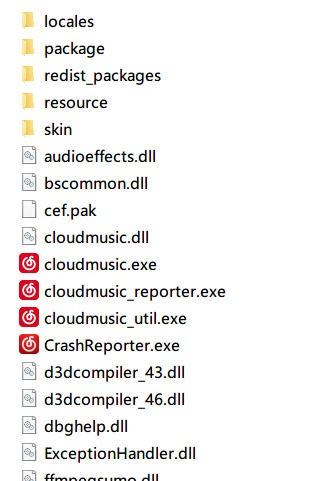
\includegraphics[width=5cm]{assets/Netease_cloud_music_files.png}
  \caption{「网易云音乐」的目录结构}
  \label{ncm-files}
\end{figure}

安装包的作用之一,便是把上面这一大堆文件按照它们能够工作的结构「释放」到我们的电脑中的指定位置。而除了「释放 app 的文件」之外,安装包还会做一些其他事情,例如设置一些文件的打开方式(上一章中提到的那张「表」)、调整一些系统内部的参数等。可以说,软件安装的过程,不仅仅是将一大堆文件「释放」或者说「提取」到系统中的某一个位置的过程,它还会对系统进行或多或少的调教与更改。这就是「安装包」存在的意义——它帮助我们完成了这复杂的「安装」过程。

\section{如何上网寻找软件的安装包}

下面我们来探讨如何上网寻找我们需要的软件的安装包。

\subsection{优先考虑:官方网站}

当要获取一款 app 时,我们首先应该考虑的是 app 开发者的官方网站,即「官网」。比起在其他地方下载软件,从官网下载软件能最大限度地保证你所下载的东西是干净的。

然而,\regcolor{对于百度这样的搜索引擎,官网常常不是搜索结果中的第一个——百度搜索出来的前 3 条结果一般是广告}。例如,我们想要下载「WPS」,直接在百度中搜索「WPS 下载」,我们会得到图 \ref{baidu-wps-result} 那样的搜索结果。

\begin{figure}[htb!]
  \centering
  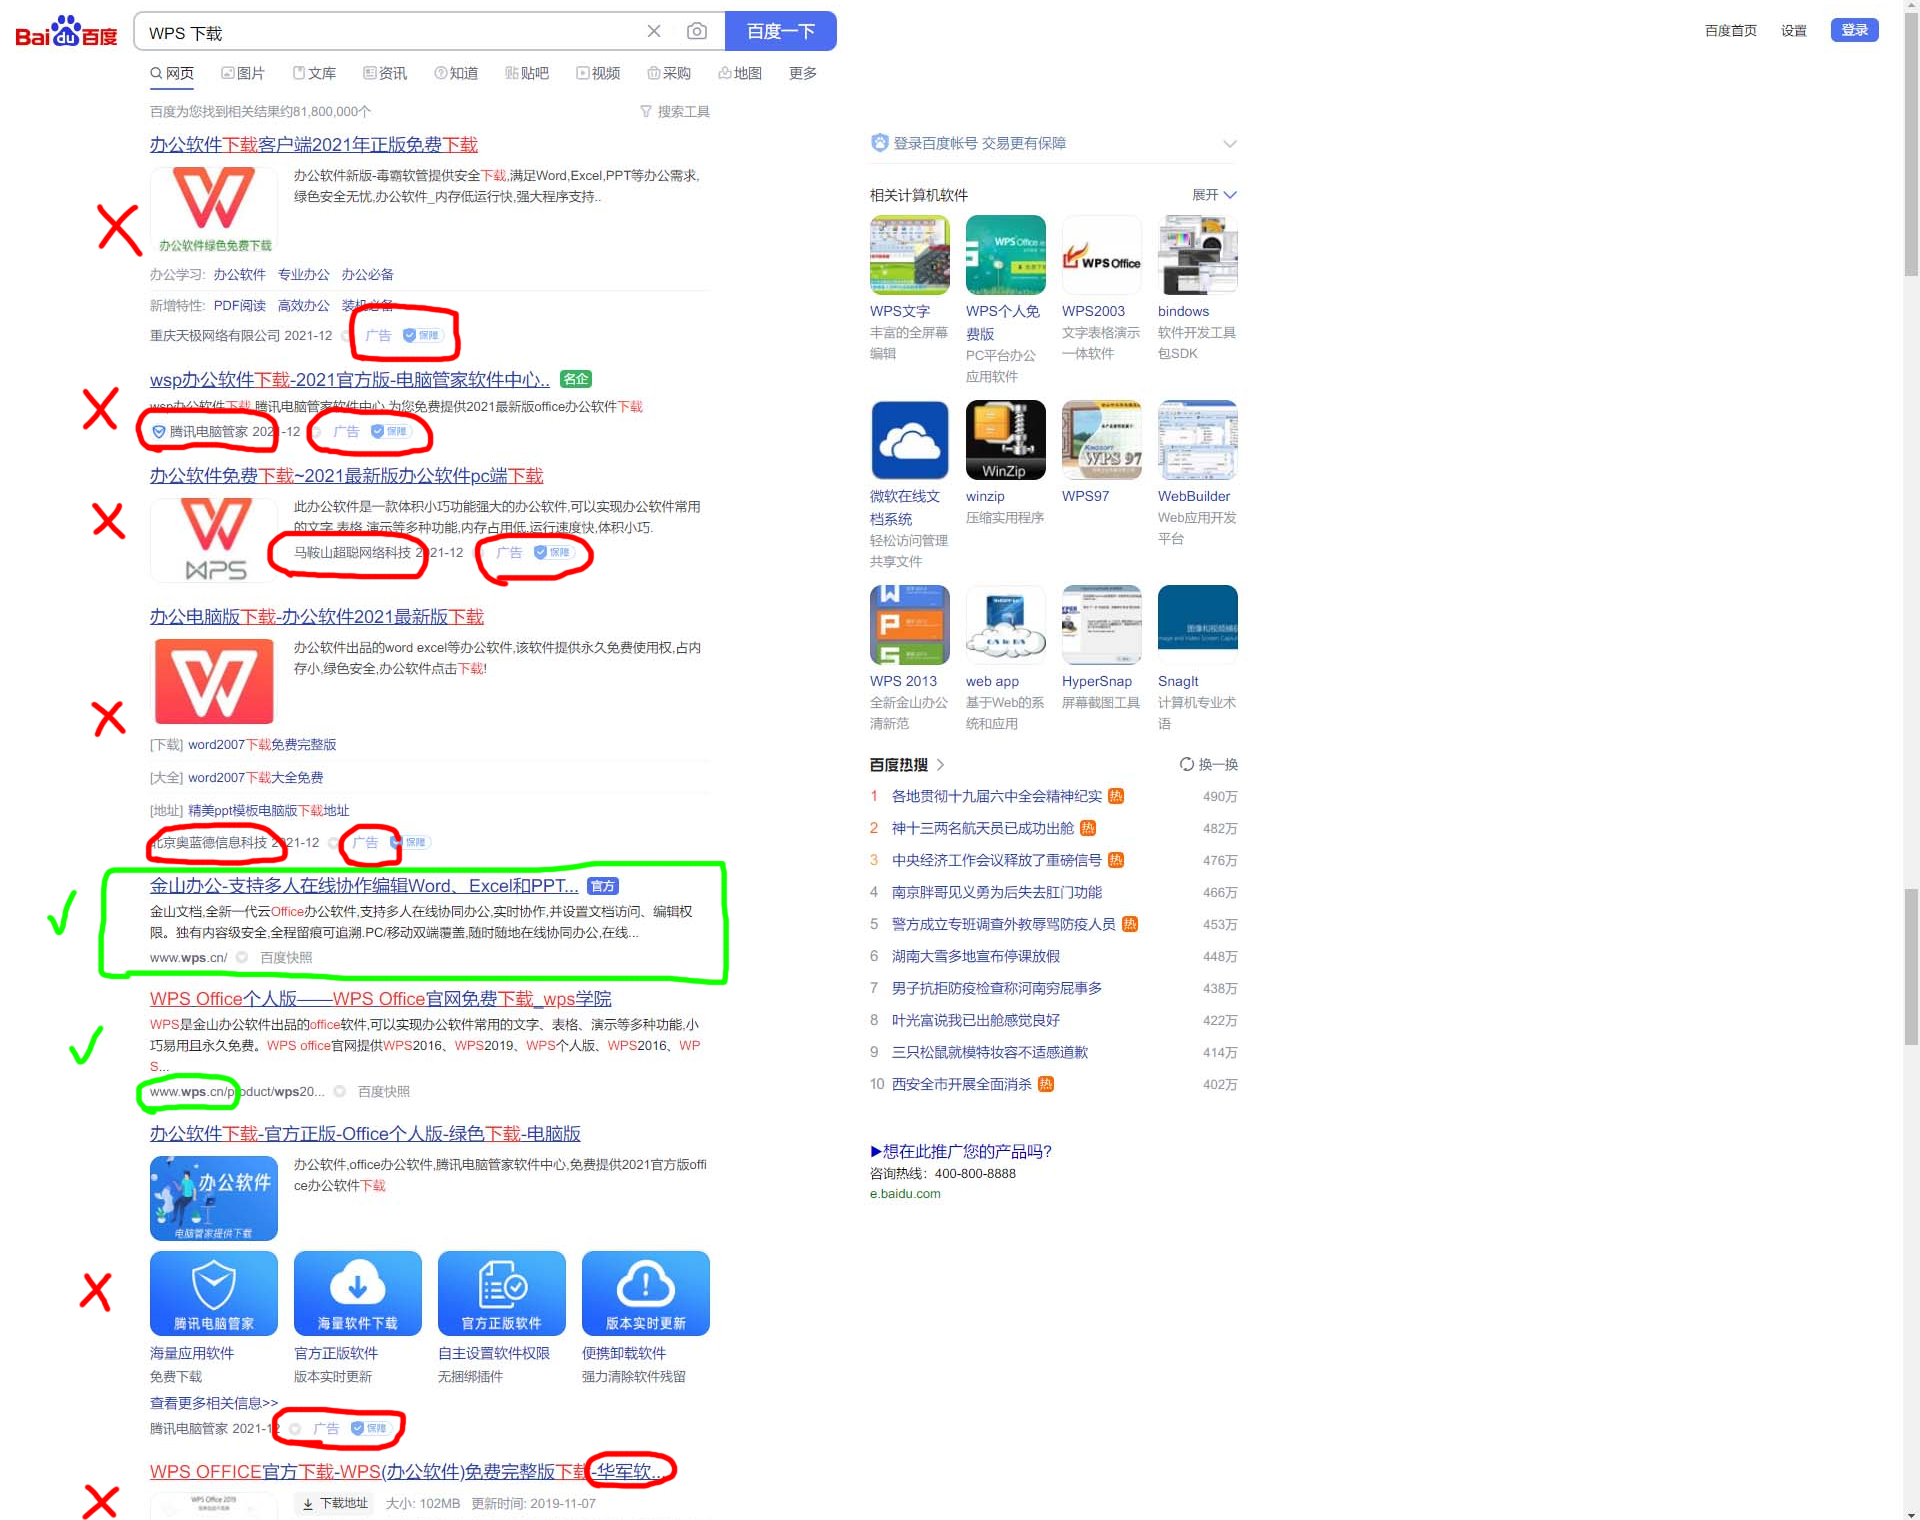
\includegraphics[width=10cm]{assets/Baidu_result.png}
  \caption{百度搜索「WPS 下载」的搜索结果}
  \label{baidu-wps-result}
\end{figure}

在图 \ref{baidu-wps-result} 中,我们搜索「WPS 下载」,然而在结果中:

\begin{itemize}
  \item 第一条是「重庆天极网络有限公司」提供的广告。
  \item 第二条是「腾讯电脑管家」提供的广告,进去之后八成你会下载到「腾讯电脑管家」而不是「WPS」。
  \item 第三条是「马鞍山超聪网络科技」提供的广告。
  \item 第四条是「北京奥蓝德信息科技」提供的广告。
\end{itemize}

\regcolor{上面这四条全部是广告}。这意味着进入这些页面,你八成下载不到干净的「WPS」,而只能下载到一堆垃圾。

\begin{itemize}
  \item 第五条是 WPS 官网。注意看它的网址是 \verb|www.wps.cn|,这是 WPS 的官方网站。
  \item 第六条也是官网。
  \item 第七条又是「腾讯电脑管家」的广告。
  \item 第八条是第三方下载站「华军软件园」的链接。我们在后面会提到,当官网不可用的时候,怎么从这种第三方下载站下载软件。
\end{itemize}

鉴别一个网站到底是不是官网,我们主要可以观察这么几个地方:

\begin{itemize}
  \item 看网址。一般官网的网址都是企业或者软件的名字。例如:
  \begin{itemize}
    \item WPS 的官网是 \verb|www.wps.cn|。
    \item QQ 的官网是 \verb|im.qq.com|。微信的则是 \verb|weixin.qq.com|。(腾讯首页:\verb|qq.com|)
    \item 网易云音乐的官网是 \verb|music.163.com|。(网易官网:\verb|163.com|)
    \item ……
  \end{itemize}
  \item 排除法。没有哪个软件厂商的名字是叫做「xx 软件站」「xx 下载站」「xx 软件园」的。带有这些名字的全部是第三方下载站。
  \item 语义判断。一般广告网站的标题都与搜索关键词没有任何实质上的联系。我们不妨再看上面的搜索结果中的前四条广告:
  \begin{itemize}
    \item 第一条:「办公软件下载客户端 2021 年正版免费下载」,只字不提「WPS」或者「金山办公」。(WPS 是金山公司开发的办公软件)
    \item 第二条:「wsp 办公软件下载-2021 官方版-电脑管家软件中心」,挂羊头卖狗肉而且挂错了。
    \item 第三条、第四条类似第一条。
  \end{itemize}
\end{itemize}

进入软件的官方网站之后,我们搜索「全部产品」「软件下载」之类的选项,就可以找到我们所需要的软件的安装包。例如从 WPS 的官网上下载 WPS 软件:

\begin{figure}[htb!]
  \centering
  
\includegraphics[width=10cm]{assets/Download_WPS.png}
  \caption{从官网下载 WPS}
  \label{download-wps}
\end{figure}

\subsection{直面深渊:第三方软件站}

在某些时候,我们确实找不到一个软件的官网,或者因为这样那样的原因不能去官网下载某个软件。这时,我们将不得不直面深渊,进入「xx 软件园」「xx 软件站」「xx 下载站」这样的网站下载软件。

这种网站一般是可以下载到我们想要的东西的——前提是,你足够小心,不点到那些所谓「高速下载器」「P2P 下载器」的虚假链接。下面我们会手把手实操这个过程。

假设我们要下载「SecureCRT」这款软件。我们在百度上搜索「SecureCRT 下载」,并主动避开那些明显骗人的广告,点击了这个看似还能接受的「华军软件园」网站:

\begin{figure}[H]
  \centering
  
\includegraphics[width=8cm]{assets/Huajun_1.png}
  \caption{「华军软件园」上的「SecureCRT」}
  \label{huajun-1}
\end{figure}

重点来了:\regcolor{进入这个网站,请主动避开所有「高速下载」「极速下载」「P2P 极速下载」这样的按钮,选择「普通下载」「本地下载」这样的按钮}:

\begin{figure}[H]
  \centering
  
\includegraphics[width=10cm]{assets/Huajun_2.png}
  \caption{不要选择【高速下载】,选择【本地下载】}
  \label{huajun-2}
\end{figure}

点击之后我们会跳转到这样一个「下载地址」的页面。同样地,我们\regcolor{不要点击「需优先下载高速下载器」之下的所有连接,而要点击「普通下载地址」下方的「通用网络下载」或者「电信网络下载」}:

\begin{figure}[H]
  \centering
  
\includegraphics[width=8cm]{assets/Huajun_3.png}
  \caption{不要点击「需优先下载高速下载器」之下的所有链接,选择「普通下载地址」下方的链接}
  \label{huajun-3}
\end{figure}

使用下方两个链接下载到的文件如图 \ref{real-securecrt},体积约 50 MB,符合这个软件的体量;它是一个压缩包,一般解压缩之后就能得到软件的安装包。而使用上方所谓「高速下载」下载到的文件是 \ref{fake-securecrt},体积只有 1 MB,而且是一个不明的「可执行文件」(exe 文件),这是不正常的。在本章的最后,我们会使用一台虚拟机来演示这「高速下载器」会干什么。

\begin{figure}[htb!]
  \centering
  \begin{minipage}{6cm}
    \centering
    
\includegraphics[width=5cm]{assets/Real_SecureCRT.png}
    \caption{点击「普通下载」得到的真正的软件安装包}
    \label{real-securecrt}
  \end{minipage}
  \qquad
  \begin{minipage}{6cm}
    \centering
    
\includegraphics[width=5cm]{assets/Fake_SecureCRT.png}
    \caption{点击「高速下载」得到的假的软件安装包}
    \label{fake-securecrt}
  \end{minipage} 
\end{figure}

\subsection{另辟蹊径:软件公众号及其他小众渠道}

另一种「另辟蹊径」的方法,是通过一些「小众渠道」,例如一些分享软件的微信公众号来下载软件。这不失为一种好方法——那些人们口口相传的优质公众号一般会把常用软件的「干净」安装包分门别类地整理分享,与「xx 下载站」相比,免去了「高速下载器」的烦恼。

但是,这种公众号一般软件不是特别多——你总有一天没法从它们那里找到想要的软件。此外,这些公众号一般使用百度网盘来分享文件,而众所周知百度网盘是对非会员限速的,这必然对使用体验有一定影响。不过总的来说,这依然是一种值得推荐的方法。

\begin{note}
  对于这类公众号,我们并没有做太多的收集,因此无法在此推荐。大家可以在 B 站、贴吧、微博等地方自行寻路。
\end{note}

\subsection{他山之石:第三方的「软件管家」}

除了手动在网上——无论是在官网,从第三方下载站,还是从那些整理网站的公众号上——下载软件的安装包之外,有一些第三方的「软件管家」也能帮助我们找到所需要的软件。这些软件管家有的是电脑厂商所维护的,例如「联想软件管家」「华为软件管家」;有的是一些公司所维护的,比如「360 软件管家」「腾讯软件管家」等(名字不一定是这样,可以类比)。

一般来说,那些由电脑厂商所维护的「软件管家」,往往相对干净、不带「全家桶」式的捆绑;而那些第三方企业维护的「软件管家」,一般都会或多或少地提示用户安装它们的「全家桶」。比如,如果你使用「360 软件管家」,那它一定会用某些手段提示用户去安装「360 安全卫士」以及一系列其他软件。因此,你可以根据自身机器的实际情况,按需选择这样的「软件管家」类 app。

\section{安装软件}

假设经过与流氓网站的「斗智斗勇」,你成功地下载到了某款软件的安装包。取决于软件,你下载到的可能是下面三种文件中的某一种:

\begin{itemize}
  \item 一个光秃秃的 \verb|exe| 文件。
  \item 一个压缩包,例如 \verb|zip| 或 \verb|rar| 文件。
  \item 一个扩展名是 \verb|iso| 的文件。
\end{itemize}

对于第一种情况,我们直接双击这个 \verb|exe| 文件就能启动安装进程。对于第二种情况,我们需要解压缩这个压缩包到某处,然后在解压出来的文件中找到名字类似「\verb|setup.exe|」或「\verb|install.exe|」的程序双击打开。对于第三种情况,我们右击这个 \verb|iso| 文件,选择【打开方式】→【文件资源管理器】,然后在弹出的新窗口中找到名字类似「\verb|setup.exe|」或「\verb|install.exe|」的程序双击打开\footnote{当你这样打开 \texttt{iso} 文件后,这个文件会临时被「映射」成电脑里的一个新「分区」,打开【此电脑】就能发现它。在你安装完成后,可以打开【此电脑】,右键这个分区选择【弹出】来让这个分区消失。}。

启动安装器后,我们一般按提示【下一步】操作即可完成安装。

\begin{note}
  此过程中也要留心!跨过了「高速下载器」的坎,可不要又掉进了捆绑软件的坑。有一些软件在安装程序中也会像「高速下载器」一样勾选了一些捆绑软件、浏览器主页劫持什么的,这些选项可能出现在安装过程中的任何阶段,一定要注意取消勾选再进行下一步。
\end{note}

在安装过程中需要特别注意的一件事,便是「软件安装位置」,即安装包把软件自身的各种文件「释放」的位置。

在上一章中我们提到过,不要把大量的软件安装在 C 盘——安装到 D 盘或其他磁盘分区是更好的选择。一般来说,软件默认会把自己「释放」在以下两个路径之一:

\begin{verbatim}
  C:\Program Files\<厂商名字>\<软件名字>
  C:\Program Files (x86)\<厂商名字>\<软件名字>
\end{verbatim}

在上一章中我们提到了「快捷方式」,在你的电脑桌面上就有许多软件可执行文件的快捷方式。右键它们选择【属性】,你就能看到这些已经安装的软件的位置。看看它们中的一些是不是在 \verb|C:\Program Files\| 或者 \verb|C:\Program Files (x86)| 下?

\verb|Program Files| 和 \verb|Program Files (x86)| 这两个文件夹,即是系统预置的两个用来安装 app 的文件夹,都位于 C 盘根目录下。然而,我们希望把软件安装到 D 盘。这里推荐一个简单好用的方法:直接将默认路径中的 \verb|C:| 改成 \verb|D:|。例如:

\begin{verbatim}
  D:\Program Files (x86)\Tencent\QQ
\end{verbatim}

这就是在 D 盘安装 QQ 软件的一个很合适的路径。这样做能保持一个比较干净的目录结构。你的 D 盘下会因此多出 \verb|Program Files| 和 \verb|Program Files (x86)| 这样的两个文件夹,用来专门在 D 盘安装软件。

\begin{figure}[htb!]
  \centering
  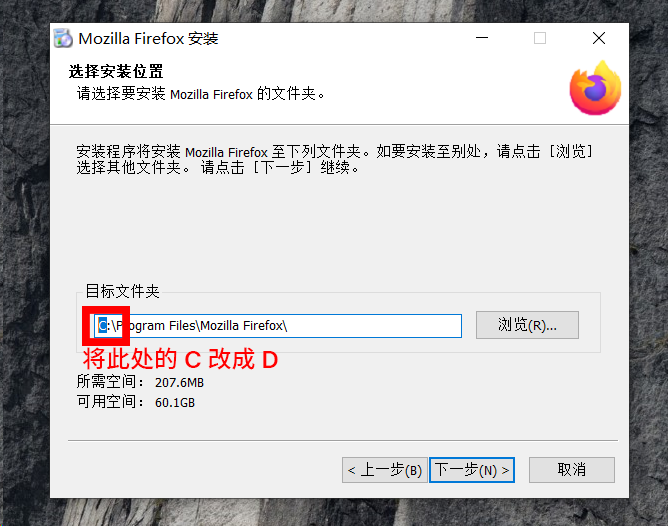
\includegraphics[width=8cm]{assets/Change_C_to_D.png}
  \caption{一般把这个 \texttt{C:} 改成 \texttt{D:} ,就能得到一个不错的 D 盘安装软件的路径}
  \label{change-c-to-d}
\end{figure}

如图 \ref{sogou-install} 所示,有一些软件的安装包不是「下一步」型的,而只有一个「立即安装」的按钮。一般这种情况,可以展开「自定义安装」之类的选项,然后更改软件的安装位置。

\begin{figure}[htb!]
  \centering
  
\includegraphics[width=8cm]{assets/Sogou_change_directory.png}
  \caption{对于只有一个「立即安装」按钮的安装包,一般找到「自定义安装」的选项展开后即可更改安装位置}
  \label{sogou-install}
\end{figure}

\section{软件收费、破解和自由软件}

很多软件是需要购买的,包括 Windows 系统本身(一般你购买电脑时,电脑厂商已经帮你出了买 Windows 这部分钱)。常见的专业软件,从平面设计领域的 Adobe 家族的 Photoshop、Premiere Pro,工程领域的 Autodesk 家族的 AutoCAD、3ds MAX,到开发领域的 JetBrains 家族的 IDEA、PyCharm,甚至于我们每天都在用的 Word 和 PowerPoint,这些软件全部都需要付费购买。图 \ref{buy-adobe} 是购买正版 Photoshop(俗称的 PS)软件的页面——定价 888 元一年。

\begin{figure}[htb!]
  \centering
  
\includegraphics[width=6cm]{assets/Adobe.png}
  \caption{Adobe 的「Creative Cloud 中国摄影计划」套装,包含 Photoshop 和 Lightroom Classic 两款软件,定价 888 元一年。}
  \label{buy-adobe}
\end{figure}

而由于这样或那样的原因,我们在实际生活中,或多或少都在「没有付费而白嫖这些软件」。这是因为我们使用的这些软件被「破解」了。破解之后,软件的计费功能失效,原本收费的软件通过某种方式变成了可以免费永久使用的软件。大体上,网上流传的破解软件一般有这么两种形式:

\begin{itemize}
  \item 一种是已经完全破解了的收费软件。这种软件已经经过修改,安装包往往也是民间自行制作的,可以直接走正常流程安装,安装后打开就可以无限制地使用。例如一些 Adobe 软件破解版套装。
  \item 另一种是使用收费软件的试用版本安装软件,再外加「破解补丁」。这种软件的安装包依然是使用官方原版的安装包,安装完成之后,通过某种「打补丁」的方式来外挂「欺骗」这官方原版的软件,让原版软件以为用户已经购买,从而解锁全部的功能并让用户无限制使用。常见的 Office 软件的破解、Autodesk 软件的破解都属于此类。
\end{itemize}

使用破解软件终究是一件「上不得台面」的事情。一般来说,如果你使用破解软件作为私下的个人使用、学习,软件厂商大多是不会进行追究的。但是,如果你将破解软件(或者说,盗版软件)用于商业用途,那必然迟早会受到追究。尽管实际生活中软件厂商维权的积极程度各有差异,尽管大家会因为各种各样的原因不得不去使用盗版和破解,但我们仍然呼吁大家支持正版软件,万不得已使用盗版、破解软件时,仅作为非商业的个人和学习用途。

与那些用来盈利的商业软件不同,「自由软件」不仅是「免费」(Free as in `free beer')的,而且是「自由」(Free as in `free speech')的。对于自由软件,人们不仅可以无偿使用,还能自由地复制、分发,甚至是在一定条款之下修改它们。自由软件的原始代码是公开的,下载使用是免费的,开发者是多元包容的。近些年来,自由软件作为一种新浪潮在互联网上的发展不断壮大,自由软件在越来越多的领域开始出现。

在今天,一些自由软件已经开始动摇过去一些不可或缺的商业软件的地位。我们鼓励大家在实际使用电脑的过程中,多多尝试、使用一些优质自由软件。在《Missing》的后续章节中,我们会推荐一批各个领域的优质软件,其中就有许多自由软件的身影。

\section{UWP 应用和 Microsoft Store *}

作为 Windows 亲爹的微软早在数年前就意识到,Windows 系统下一直缺少一个官方维护的、像 Apple 的 App Store 那样的「集中化」的软件中心,用户下载软件只能像上文那样上网去苦苦找寻。彼时的微软公司正打算进军手机行业,想要和安卓与 iOS 形成「三足鼎立」之势,微软于是心想:不如弄一种新的 app 格式,这种新的 app 不仅能在我们的 Windows 电脑上运行,还可以在手机上运行;然后我们再顺带弄一个全是这种新格式 app 的应用商店,可谓一举两得。于是微软就这么干了:这种新的 app 格式叫做「通用 Windows 平台应用」(Universal Windows Platform,简称「UWP 应用」),这个应用商店就是我们电脑里的「Microsoft Store」:

\begin{figure}[H]
  \centering
  \includegraphics[width=5cm]{assets/MS_Store_1.png}
  \caption{Windows 10 中的 Microsoft Store}
  \label{ms-store-in-windows-10}
\end{figure}

可是,时过境迁:微软终究没有能在手机市场打下一片江山,微软做的手机系统最终在近两年宣布「谢幕」。可是微软心想,这「UWP 应用」的先进构想和 Microsoft Store 不能开了头就没了尾,因此它们直到今天依然被保留在 Windows 系统之中。

如果你有打开过「Microsoft Store」,如图 \ref{ms-store},你会发现,其中有一些应用是我们日常生活中的常用应用,而另外的大多数应用,我们都从来没有听说过。而事实上,如果你去仔细查看那里面的常用应用,会发现它们往往更新得没有官网勤快,有些甚至已经停止了更新。

\begin{figure}[htb!]
  \centering
  \includegraphics[width=10cm]{assets/MS_Store_2.png}
  \caption{Microsoft Store 的界面}
  \label{ms-store}
\end{figure}

事实上,这就是 Microsoft Store 的现状:作为推广「UWP 应用」的第一线,它没有什么很拿得出手的「杀手锏」;作为一个「xxx 软件中心」的替代品,它的应用相当不全。微软在 Microsoft Store 和 UWP 应用上充满了雄心壮志,却最终落得今天的结局。

\section{演示:「高速下载器」到底会干什么}

\begin{note}
  \textbf{请不要在自己电脑上尝试打开这种「高速下载器」!}
\end{note}

在上文中我们演示下载「SecureCRT」时,如果点选了「高速下载」,会得到如图 \ref{gao-su-downloader-1} 的一个只有 1 MB 的可执行文件:

\begin{figure}[H]
  \centering
  \includegraphics[width=5cm]{assets/Gao_su_1.png}
  \caption{下载到的「高速下载器」,一般来说体积在 1 MB 左右}
  \label{gao-su-downloader-1}
\end{figure}

双击这个「高速下载器」,弹出的窗口如图 \ref{gao-su-downloader-2}。可以看到,右方有四个捆绑软件的复选框被默认勾选:「360 安全浏览器」「QQ 游戏大厅」「U 号租」「百度网盘」,右下方还有一个「六间房直播」。假设我们足够理智,取消勾选了这里的所有的勾,然后点击「快速安装」。等待进度条跑完之后,则会来到图 \ref{gao-su-downloader-3} 的界面。这个界面上又有两个软件捆绑「绝地求生」和「傲视霸主」,以及一个「使用 360 安全导航」的复选框。

\begin{figure}[htb!]
  \centering
  \begin{minipage}{6cm}
    \centering
    \includegraphics[width=5cm]{assets/Gao_su_2.png}
    \caption{「高速下载器」打开后的界面}
    \label{gao-su-downloader-2}
  \end{minipage}
  \qquad
  \begin{minipage}{6cm}
    \centering
    \includegraphics[width=5cm]{assets/Gao_su_3.png}
    \caption{「高速下载器」完成下载后的界面}
    \label{gao-su-downloader-3}
  \end{minipage} 
\end{figure}

全部取消这些复选框,我们点击「打开文件」,终于打开了我们想要的 SecureCRT 的安装包——一个名为 SecureCRT.rar 的,体积约 50 MB 的压缩包。而这就是我们直接点选「普通下载」直接就能下载到的东西。

如果我们没有取消上面的这些勾选,那会是什么结局呢?

\begin{note}
  \regcolor{警告:请勿模仿!}
\end{note}

\begin{figure}[H]
  \centering
  \begin{minipage}{8cm}
    \centering
    \includegraphics[width=7cm]{assets/Gao_su_4.png}
    \caption{被乱七八糟的软件「占领」的电脑桌面}
    \label{gao-su-downloader-4}
  \end{minipage}
  \qquad
  \begin{minipage}{4cm}
    \centering
    \includegraphics[width=3cm]{assets/Gao_su_5.png}
    \caption{充满各种乱七八糟的软件的「开始」菜单}
    \label{gao-su-downloader-5}
  \end{minipage} 
\end{figure}

我们得到的结论是:

所谓「高速下载器」最后下载到的就是你点击「普通下载」得到的东西,纯属脱裤子放屁。

而「高速下载器」在整个过程中带有许多的捆绑勾选,一旦不留神你的电脑就会被各种垃圾软件充斥。

\begin{note}
  这种流氓的「高速下载器」一般被戏称为「高速下崽器」。
\end{note}

\practice

\begin{enumerate}
  \item 在图 \ref{how-to-download-it-1} 至图 \ref{how-to-download-it-3} 中,怎样操作最不可能下载到垃圾?
  \begin{figure}[htb!]
    \centering
    \begin{minipage}{8cm}
      \centering
      \includegraphics[width=7cm]{assets/How_to_1.png}
      \caption{下载软件「谷歌浏览器」}
      \label{how-to-download-it-1}
    \end{minipage}
    \qquad
    \begin{minipage}{4cm}
      \centering
      \includegraphics[width=3cm]{assets/How_to_2.png}
      \caption{下载软件「QQ」}
      \label{how-to-download-it-2}
    \end{minipage}    
    \\
    \vspace{1ex}
    \begin{minipage}{12cm}
      \centering
      \includegraphics[width=10cm]{assets/How_to_3.png}
      \caption{下载软件「WPS」}
      \label{how-to-download-it-3}
    \end{minipage}
  \end{figure}
  \item 图 \ref{how-to-download-it-4} 的界面中有几个捆绑勾选?
  \begin{figure}[htbp]
    \centering
    \includegraphics[width=8cm]{assets/How_to_4.png}
    \caption{下载「微信电脑版」时不慎下载到的「高速下载器」}
    \label{how-to-download-it-4}
  \end{figure}
  \item 下载「微信电脑版」,下面三个文件体积中哪一个最可能不是垃圾软件?
  \begin{enumerate}
    \item 640 KB 
    \item 1.1 MB
    \item 150 MB  
  \end{enumerate}
  \item 下面四个软件安装路径,谁最合适?其他的不合适在哪里?
  \begin{enumerate}
    \item 安装 Steam:\verb|C:\Program Files\steam|
    \item 安装微信电脑版:\verb|D:\Program Files (x86)\Tencent\Wechat|
    \item 安装 Vivado:\verb|D:\软件\Xilinx\Vivado|
    \item 安装网易云音乐:\verb|桌面\我的软件\Cloudmusic|
  \end{enumerate}
  \item 假设某个软件已经被安装在了一个地方,我现在想把这个软件放到另一个地方,可以直接剪切移动整个软件的目录到另一个地方吗?
  \item 查看自己电脑上 5 个不同软件的安装位置,并打开它们的安装目录,看一看里面的结构。
\end{enumerate}

\end{document}